\documentclass[10pt,journal,compsoc]{IEEEtran}
\usepackage[utf8]{inputenc}
\usepackage[vietnamese,english]{babel}
\usepackage{amsmath,amssymb,amsfonts}
\usepackage{algorithmic}
\usepackage{algorithm}
\usepackage{float}
\usepackage{array}
\usepackage{booktabs}
\usepackage{multirow}
\usepackage{graphicx}
\usepackage{textcomp}
\usepackage{xcolor}
\usepackage{url}
\usepackage{hyperref}
\usepackage{cite}
\hypersetup{
    colorlinks=true,
    linkcolor=blue,
    citecolor=blue,
    urlcolor=blue
}

% Enforce IEEEtran numbering schema (I, II... for sections; A, B... for subsections) against babel overrides
\addto\captionsvietnamese{%
  \renewcommand{\thesection}{\Roman{section}}%
  \renewcommand{\thesubsection}{\Alph{subsection}}%
  \renewcommand{\thesubsubsection}{\arabic{subsubsection}}%
  \renewcommand{\thesectiondis}{\Roman{section}.}%
  \renewcommand{\thesubsectiondis}{\Alph{subsection}.}%
  \renewcommand{\thesubsubsectiondis}{\arabic{subsubsection})}%
}

% Cấu hình tối ưu hóa vị trí float ngăn ngừa hiện tượng dồn bảng/hình sang các trang sau
\renewcommand{\topfraction}{0.95}
\renewcommand{\bottomfraction}{0.95}
\renewcommand{\textfraction}{0.05}
\renewcommand{\floatpagefraction}{0.85}
\renewcommand{\dbltopfraction}{0.95}
\renewcommand{\dblfloatpagefraction}{0.85}

\title{RA-HE-DLinear: Khung Dự Báo Thích Ứng Chế Độ Thị Trường và Ràng Buộc Kinh Tế Cho Nhu Cầu Du Lịch Đa Quốc Gia}

\author{Trần~Nguyễn~Tuấn,
        Phan~Hoài~Bão}

\IEEEtitleabstractindextext{%
\begin{abstract}
Dự báo nhu cầu du lịch đa quốc gia gặp nhiều thách thức do tính mùa vụ, thay đổi cấu trúc của thị trường và sự khác biệt về động lực giữa các quốc gia. Các mô hình dự báo chuỗi thời gian tuyến tính có ưu điểm về chi phí tính toán nhưng thường chưa khai thác đầy đủ biến ngoại sinh, thông tin về trạng thái thị trường và phụ thuộc giữa các quốc gia. Nghiên cứu này đề xuất RA-HE-DLinear (\textit{Regime-Aware Hierarchical-Economic DLinear}), một khung dự báo kết hợp mô hình hóa trạng thái thị trường, biến ngoại sinh, phụ thuộc liên quốc gia và ràng buộc kinh tế trong một quy trình thống nhất. Cơ chế Conformal Prediction được sử dụng để lượng hóa độ bất định, trong khi SHAP được áp dụng để phân tích đóng góp của các đặc trưng.
Khung mô hình được đánh giá trên dữ liệu du lịch Eurostat và dữ liệu World Bank theo giao thức đánh giá theo thứ tự thời gian. Trên tập kiểm thử Eurostat, RA-HE-DLinear đạt WAPE \textbf{14,59\% $\pm$ 0,46\%} đối với lượt khách và \textbf{25,00\% $\pm$ 0,54\%} đối với số đêm lưu trú (qua 1.000 lượt bootstrap), cải thiện tương đối 46,6\% và 23,6\% so với mô hình cơ sở Seasonal Naive. Trên tập kiểm thử World Bank, mô hình đạt WAPE lượt khách \textbf{9,45\% $\pm$ 0,38\%} và WAPE số đêm \textbf{28,27\% $\pm$ 0,82\%}. Phép chiếu ràng buộc loại bỏ toàn bộ 7 trường hợp vi phạm quan sát được trong 4.712 mẫu kiểm thử, tương ứng tỷ lệ can thiệp 0,15\%. Phân tích loại bỏ thành phần và phân tích theo chế độ thị trường cho thấy thông tin trạng thái, biến ngoại sinh và phụ thuộc liên quốc gia đều có đóng góp quan trọng đối với hiệu năng dự báo.
Các kết quả cho thấy việc kết hợp mô hình hóa chế độ thị trường, phụ thuộc liên quốc gia và ràng buộc miền có thể cải thiện đồng thời độ chính xác và tính nhất quán của dự báo trong bài toán nhu cầu du lịch đa quốc gia.
\end{abstract}

\begin{IEEEkeywords}
Dự báo nhu cầu du lịch, RA-HE-DLinear, RA-Exo-DLinear, LTSF-Linear, FiLM, TRMF, ràng buộc kinh tế, Conformal Prediction.
\end{IEEEkeywords}}

\begin{document}
\selectlanguage{vietnamese}
\renewcommand{\thesection}{\Roman{section}}
\renewcommand{\thesubsection}{\Alph{subsection}}
\renewcommand{\thesubsubsection}{\arabic{subsubsection}}
\renewcommand{\thesectiondis}{\Roman{section}.}
\renewcommand{\thesubsectiondis}{\Alph{subsection}.}
\renewcommand{\thesubsubsectiondis}{\arabic{subsubsection})}
\maketitle
\IEEEdisplaynontitleabstractindextext
\IEEEpeerreviewmaketitle
\raggedbottom
\section{Giới Thiệu}
\subsection{Bối Cảnh và Động Cơ Nghiên Cứu}
\IEEEPARstart{T}{rong} lĩnh vực kinh tế du lịch và quản trị khách sạn, dự báo số lượt khách đến ($Y_{\text{arr}}$) và số đêm lưu trú ($Y_{\text{nig}}$) cung cấp thông tin phục vụ việc lập kế hoạch công suất, phân bổ nguồn lực và xây dựng chính sách quản lý điểm đến\cite{song2021tourism}. Dự báo theo đa chân trời thời gian chẳng hạn ($H \in \{3, 6, 12\}$ tháng) có thể hỗ trợ các tổ chức liên quan chuẩn bị cho biến động nhu cầu giữa mùa cao điểm và mùa thấp điểm, đồng thời chủ động ngăn ngừa quá tải hạ tầng trong mùa cao điểm.
Trải qua hơn bốn thập kỷ phát triển, các phương pháp dự báo nhu cầu du lịch đã tiến triển từ kinh tế lượng cổ điển (SARIMA, Holt-Winters) \cite{athanasopoulos2011tourism}, học máy trên dữ liệu bảng (LightGBM, CatBoost) \cite{dorogush2018catboost}, đến các mạng học sâu hồi quy và cơ chế chú ý (LSTM, Transformer) \cite{claveria2016tourism, silva2023tourism}. Gần đây, nghiên cứu của Zeng et al. (AAAI 2023) \cite{zeng2023dlinear} đã đề xuất mô hình dự báo chuỗi thời gian sử dụng phép phân rã xu thế–mùa vụ và các phép biến đổi tuyến tính. Kết quả nghiên cứu cho thấy mô hình đạt hiệu năng cạnh tranh trên một số bộ dữ liệu dự báo dài hạn. Bằng cách tách chuỗi thành thành phần xu thế ($\mathbf{X}_{\text{trend}}$) và mùa vụ ($\mathbf{X}_{\text{seasonal}}$) qua bộ lọc trung bình trượt, DLinear đã vượt qua các kiến trúc Transformer phức tạp trên nhiều tập chuẩn dự báo dài hạn (LTSF) với chi phí tính toán tối ưu.
\subsection{Bài Toán và Thách Thức Nghiên Cứu}
DLinear phân rã chuỗi đầu vào thành thành phần xu thế và thành phần mùa vụ bằng bộ lọc trung bình trượt, sau đó sử dụng các phép biến đổi tuyến tính để dự báo \cite{zeng2023dlinear}. Tuy nhiên, nó không được thiết kế  cho việc kết hợp trạng thái thị trường, biến ngoại sinh và quan hệ giữa nhiều quốc gia trong cùng một khung dự báo. Với bài toán dự báo nhu cầu du lịch đa quốc gia, nghiên cứu này tập trung vào ba vấn đề:
\begin{enumerate}
    \item \textbf{Thay đổi trạng thái thị trường:} quan hệ giữa dữ liệu quá khứ và nhu cầu tương lai có thể thay đổi giữa các giai đoạn bình thường, khủng hoảng và phục hồi.
    \item \textbf{Thông tin ngoại sinh và liên quốc gia:} lịch lễ, biến kinh tế và các mẫu biến động chung giữa các quốc gia cần được khai thác cùng với chuỗi mục tiêu.
    \item \textbf{Tính nhất quán của dự báo:} dự báo lượt khách và số đêm lưu trú cần tuân thủ ràng buộc nghiệp vụ đã xác định, đồng thời cần có thông tin về độ bất định của dự báo.
\end{enumerate}
Các vấn đề trên là động lực để xây dựng và đánh giá khung RA-HE-DLinear. Mức độ hạn chế của DLinear trong bối cảnh này được xem xét thông qua các thí nghiệm đối sánh trên dữ liệu Eurostat và World Bank, thay vì được giả định là đúng với mọi bộ dữ liệu chuỗi thời gian.
\subsection{Mục Tiêu và Đóng Góp Nghiên Cứu}
Nhằm xử lý các hạn chế trên, bài báo đề xuất khung mô hình \textbf{RA-HE-DLinear} (\textit{Regime-Aware Hierarchical-Economic DLinear}). Các đóng góp chính của nghiên cứu được tóm tắt như sau:
\begin{enumerate}
    \item \textbf{Đề xuất động cơ thời gian RA-Exo-DLinear:} Mở rộng kiến trúc phân rã xu thế--mùa vụ của DLinear bằng cơ chế Điều biến Tuyến tính theo Đặc trưng (FiLM) cho nhánh xu thế dựa trên trạng thái thị trường HMM, đồng thời bổ sung các ánh xạ tuyến tính có tham số học được cho biến lịch lễ tương lai và biến kinh tế quá khứ.
    \item \textbf{Mô hình hóa phụ thuộc liên quốc gia bằng TRMF:} Sử dụng phương pháp phân rã ma trận có điều chuẩn theo thời gian (Temporal Regularized Matrix Factorization, TRMF) để biểu diễn các mẫu biến động chung giữa các quốc gia. Khả năng phản ánh các cơ chế liên kết cụ thể, chẳng hạn trong khu vực Schengen, cần được diễn giải trong phạm vi các biến và dữ liệu thực nghiệm đã sử dụng.
    \item \textbf{Xây dựng phép hiệu chỉnh dự báo theo ràng buộc giữa lượt khách và số đêm lưu trú $\Pi_{\mathcal{C}}$:} Xây dựng toán tử chiếu mốc neo bảo đảm cận vật lý $\hat{Y}_{\text{nig}} \ge \hat{Y}_{\text{arr}}$ kết hợp hàm phạt liên kết $\mathcal{L}_{\text{cons}}$, giúp kiểm soát vi phạm tự nhiên trước chiếu ở mức 0,15\% (7/4.712 mẫu) và đưa mức lệch dải kinh tế lịch sử về 16,02\% (thay vì 49,19\% của LightGBM).
    \item \textbf{Ước lượng khoảng dự báo bằng Conformal Prediction:} Ứng dụng kỹ thuật Deep Conformal Quantile Forecasting (DCQF) thiết lập khoảng dự báo $[P_{10}, P_{90}]$ có cơ sở lý thuyết về độ bao phủ dưới các giả định tương ứng $\ge 90\%$ trên mẫu hữu hạn mà không phụ thuộc giả định phân phối chuẩn.
    \item \textbf{Đánh giá thực nghiệm trên hai bộ dữ liệu:} Đánh giá trên bảng dữ liệu tháng Eurostat (38 quốc gia) và dữ liệu năm World Bank (203 nền kinh tế) theo giao thức kiểm định không rò rỉ dữ liệu, báo cáo đầy đủ chỉ số thống kê Mean $\pm$ Std qua 1.000 lượt bootstrap, phân tích bóc tách thành phần và phân tích độ nhạy.
\end{enumerate}
\section{Các Nghiên Cứu Liên Quan}
\subsection{Dự Báo Nhu Cầu Du Lịch (Tourism Demand Forecasting)}
Các phương pháp kinh tế lượng cổ điển như SARIMA và mô hình hiệu chỉnh sai số (ECM) đã được nghiên cứu và sử dụng trong dự báo nhu cầu du lịch trong nhiều thập kỷ \cite{athanasopoulos2011tourism, song2021tourism}. Trong thập kỷ gần đây, các mô hình học máy trên dữ liệu bảng (LightGBM, CatBoost) \cite{dorogush2018catboost} và mạng nơ-ron hồi quy (LSTM) \cite{claveria2016tourism, silva2023tourism} đã được áp dụng rộng rãi nhờ khả năng phi tuyến hóa quan hệ trễ. Các mô hình này có thể khai thác quan hệ phi tuyến và thông tin trễ trong dữ liệu. Tuy nhiên, hiệu quả dự báo phụ thuộc vào cách xây dựng đặc trưng, cấu hình mô hình và đặc điểm của bộ dữ liệu. Khi chuỗi thời gian xuất hiện các thay đổi cấu trúc, cần đánh giá riêng khả năng duy trì hiệu năng của từng phương pháp.
\subsection{Dự Báo Thích Ứng Chuyển Dịch Chế Độ (Regime-Aware Forecasting)}
Hiện tượng trôi dạt khái niệm (concept drift) và đứt gãy cấu trúc (structural breaks) là thách thức phổ biến trong chuỗi thời gian kinh tế lượng \cite{clements1998forecasting}. Mô hình Markov chuyển chế độ (Markov-Switching) của Hamilton \cite{hamilton1989regime} đã thiết lập nền tảng lý thuyết vững chắc cho việc nhận diện các chu kỳ kinh tế tiềm ẩn. Gần đây, cơ chế Feature-wise Linear Modulation (FiLM) \cite{perez2018film} được đề xuất nhằm đưa thông tin điều kiện bối cảnh vào mạng nơ-ron mà không làm tăng độ sâu cấu trúc. Việc kết hợp mô hình chuyển chế độ với kiến trúc phân rã tuyến tính để điều chỉnh nhánh xu thế là hướng tiếp cận mà nghiên cứu này xem xét. Mức độ mới và khác biệt của sự kết hợp này cần được xác lập thông qua đối chiếu có hệ thống với các công trình liên quan.
\subsection{Dự Báo Đa Biến và Lan Tỏa Liên Quốc Gia (Cross-Country Forecasting)}
Trong các thị trường du lịch liên kết chặt chẽ như khu vực Schengen Châu Âu, dòng khách du lịch giữa các quốc gia có sự phụ thuộc lan tỏa không gian rõ rệt. Các mô hình mạng nơ-ron đồ thị không -- thời gian (Spatio-Temporal GNN) đòi hỏi ma trận kề cố định dựa trên khoảng cách địa lý, vốn khó phản ánh đúng mạng lưới hàng không giá rẻ. Phương pháp phân rã ma trận có điều chuẩn theo thời gian (TRMF \cite{yu2016trmf}) giải quyết hạn chế này bằng cách bóc tách các nhân tố tiềm ẩn thông qua phân rã ma trận thấp chiều kèm điều chuẩn tự hồi quy. Tuy nhiên, việc mô hình hóa quan hệ liên quốc gia thường thiếu sự kết hợp đồng bộ với các ràng buộc nghiệp vụ nội tại giữa các chỉ tiêu du lịch.
\subsection{Lượng Hóa Độ Bất Định và Khả Năng Giải Thích (Uncertainty and Explainability)}
Dự báo điểm đơn thuần không đủ thông tin cho công tác quản trị rủi ro du lịch. Conformal Prediction \cite{vovk2005algorithmic, angelopoulos2021conformal} cung cấp khung mô hình lượng hóa độ bất định phi phân phối với bảo chứng độ bao phủ trên mẫu hữu hạn. Đồng thời, kỹ thuật giải thích mô hình SHAP (SHapley Additive exPlanations \cite{lundberg2017shap}) giúp bóc tách tầm quan trọng của từng thuộc tính dự báo. Từ các nghiên cứu được tổng quan, bài báo tập trung đánh giá việc kết hợp dự báo nhu cầu, hiệu chỉnh theo ràng buộc giữa số lượt khách và số đêm lưu trú, cùng lượng hóa độ bất định trong một quy trình thống nhất. Điểm cần kiểm chứng là liệu sự kết hợp này có cải thiện độ chính xác và tính nhất quán của dự báo so với các cấu hình không sử dụng đầy đủ những thành phần trên hay không.
\section{Phương Pháp Nghiên Cứu}
\subsection{Phát Biểu Bài Toán và Ký Hiệu Hình Thức}
Xét bảng dữ liệu du lịch gồm $N$ quốc gia quan sát qua thời gian $t = 1, \dots, T$. Tại mỗi thời điểm $t$ và quốc gia $i$, biến mục tiêu là véc-tơ hai chiều $\mathbf{y}_{i, t} = [Y_{i, t}^{\text{arr}}, Y_{i, t}^{\text{nig}}]^T \in \mathbb{R}_+^2$, tương ứng với lượt khách đến và số đêm lưu trú. Cho trước cửa sổ quan sát quá khứ độ dài $L$ và chân trời dự báo $H$, bài toán đặt ra là ước lượng:
\begin{equation}
\begin{aligned}
\hat{\mathbf{Y}}_{i, t+1:t+H} = \mathcal{M}\big( & \mathbf{Y}_{i, t-L+1:t}, \, \mathbf{X}_{i, t-L+1:t}^{\text{past}}, \\
& \mathbf{X}_{i, t+1:t+H}^{\text{fut}}, \, \mathbf{s}_t\big)
\end{aligned}
\end{equation}
thỏa mãn đồng thời hai mục tiêu: tối thiểu hóa sai số dự báo và tuân thủ ràng buộc kinh tế:
\begin{equation}
\hat{Y}_{i, \tau}^{\text{nig}} \ge \hat{Y}_{i, \tau}^{\text{arr}} \times \text{LOS}_{\min}, \quad \forall \tau \in [t+1, t+H]
\end{equation}
với $\text{LOS}_{\min} = 1$ đêm.
\begin{table}[!htbp]
\centering
\caption{Bảng ký hiệu toán học chính trong bài báo}
\label{tab:notations}
\small
\setlength{\tabcolsep}{3pt}
\renewcommand{\arraystretch}{1.0}
\begin{tabular}{p{2.35cm}p{6.05cm}}
\toprule
\textbf{Ký hiệu} & \textbf{Ý nghĩa toán học} \\
\midrule
$L, H$ & Độ dài chuỗi dữ liệu quá khứ (lookback) và khoảng dự báo (forecast horizon) \\
$N, C$ & Số lượng quốc gia ($N$) và số lượng biến mục tiêu ($C=2$) \\
$K_{\text{ma}}$ & Kích thước cửa sổ trung bình trượt dùng để tách thành phần xu thế \\
$\mathbf{X}_{\text{trend}}, \mathbf{X}_{\text{seasonal}}$ & Thành phần xu thế chu kỳ và mùa vụ nội sinh \\
$\mathbf{X}_{\text{fut}}, \mathbf{X}_{\text{past}}$ & Ma trận biến ngoại sinh lịch lễ tương lai và kinh tế quá khứ \\
$s_t \in \{0, 1, 2\}$ & Trạng thái chế độ thị trường tiềm ẩn từ Gaussian HMM \\
$\mathbf{e}_r \in \mathbb{R}^{d_r}$ & Véc-tơ nhúng không gian liên tục của chế độ thị trường \\
$\alpha_{\text{trend}}, \alpha_{\text{fut}}, \alpha_{\text{past}}$ & Hệ số tỷ lệ co giãn học được của các luồng đặc trưng \\
$\mathbf{W}, \mathbf{X}_{\text{sp}}$ & Ma trận nhân tố không gian và thời gian trong mô hình TRMF \\
$\Pi_{\mathcal{C}}$ & Toán tử chiếu lồi lên tập hợp chấp nhận được về mặt kinh tế \\
$1 - \alpha$ & Mức độ tin cậy danh định của dải conformal (90\%) \\
\bottomrule
\end{tabular}
\end{table}
\subsection{Mô Hình Đề Xuất RA-HE-DLinear}
Hình~\ref{fig:architecture} minh họa quy trình hoạt động toàn diện của khung RA-HE-DLinear.
\begin{figure*}[!t]
\centering
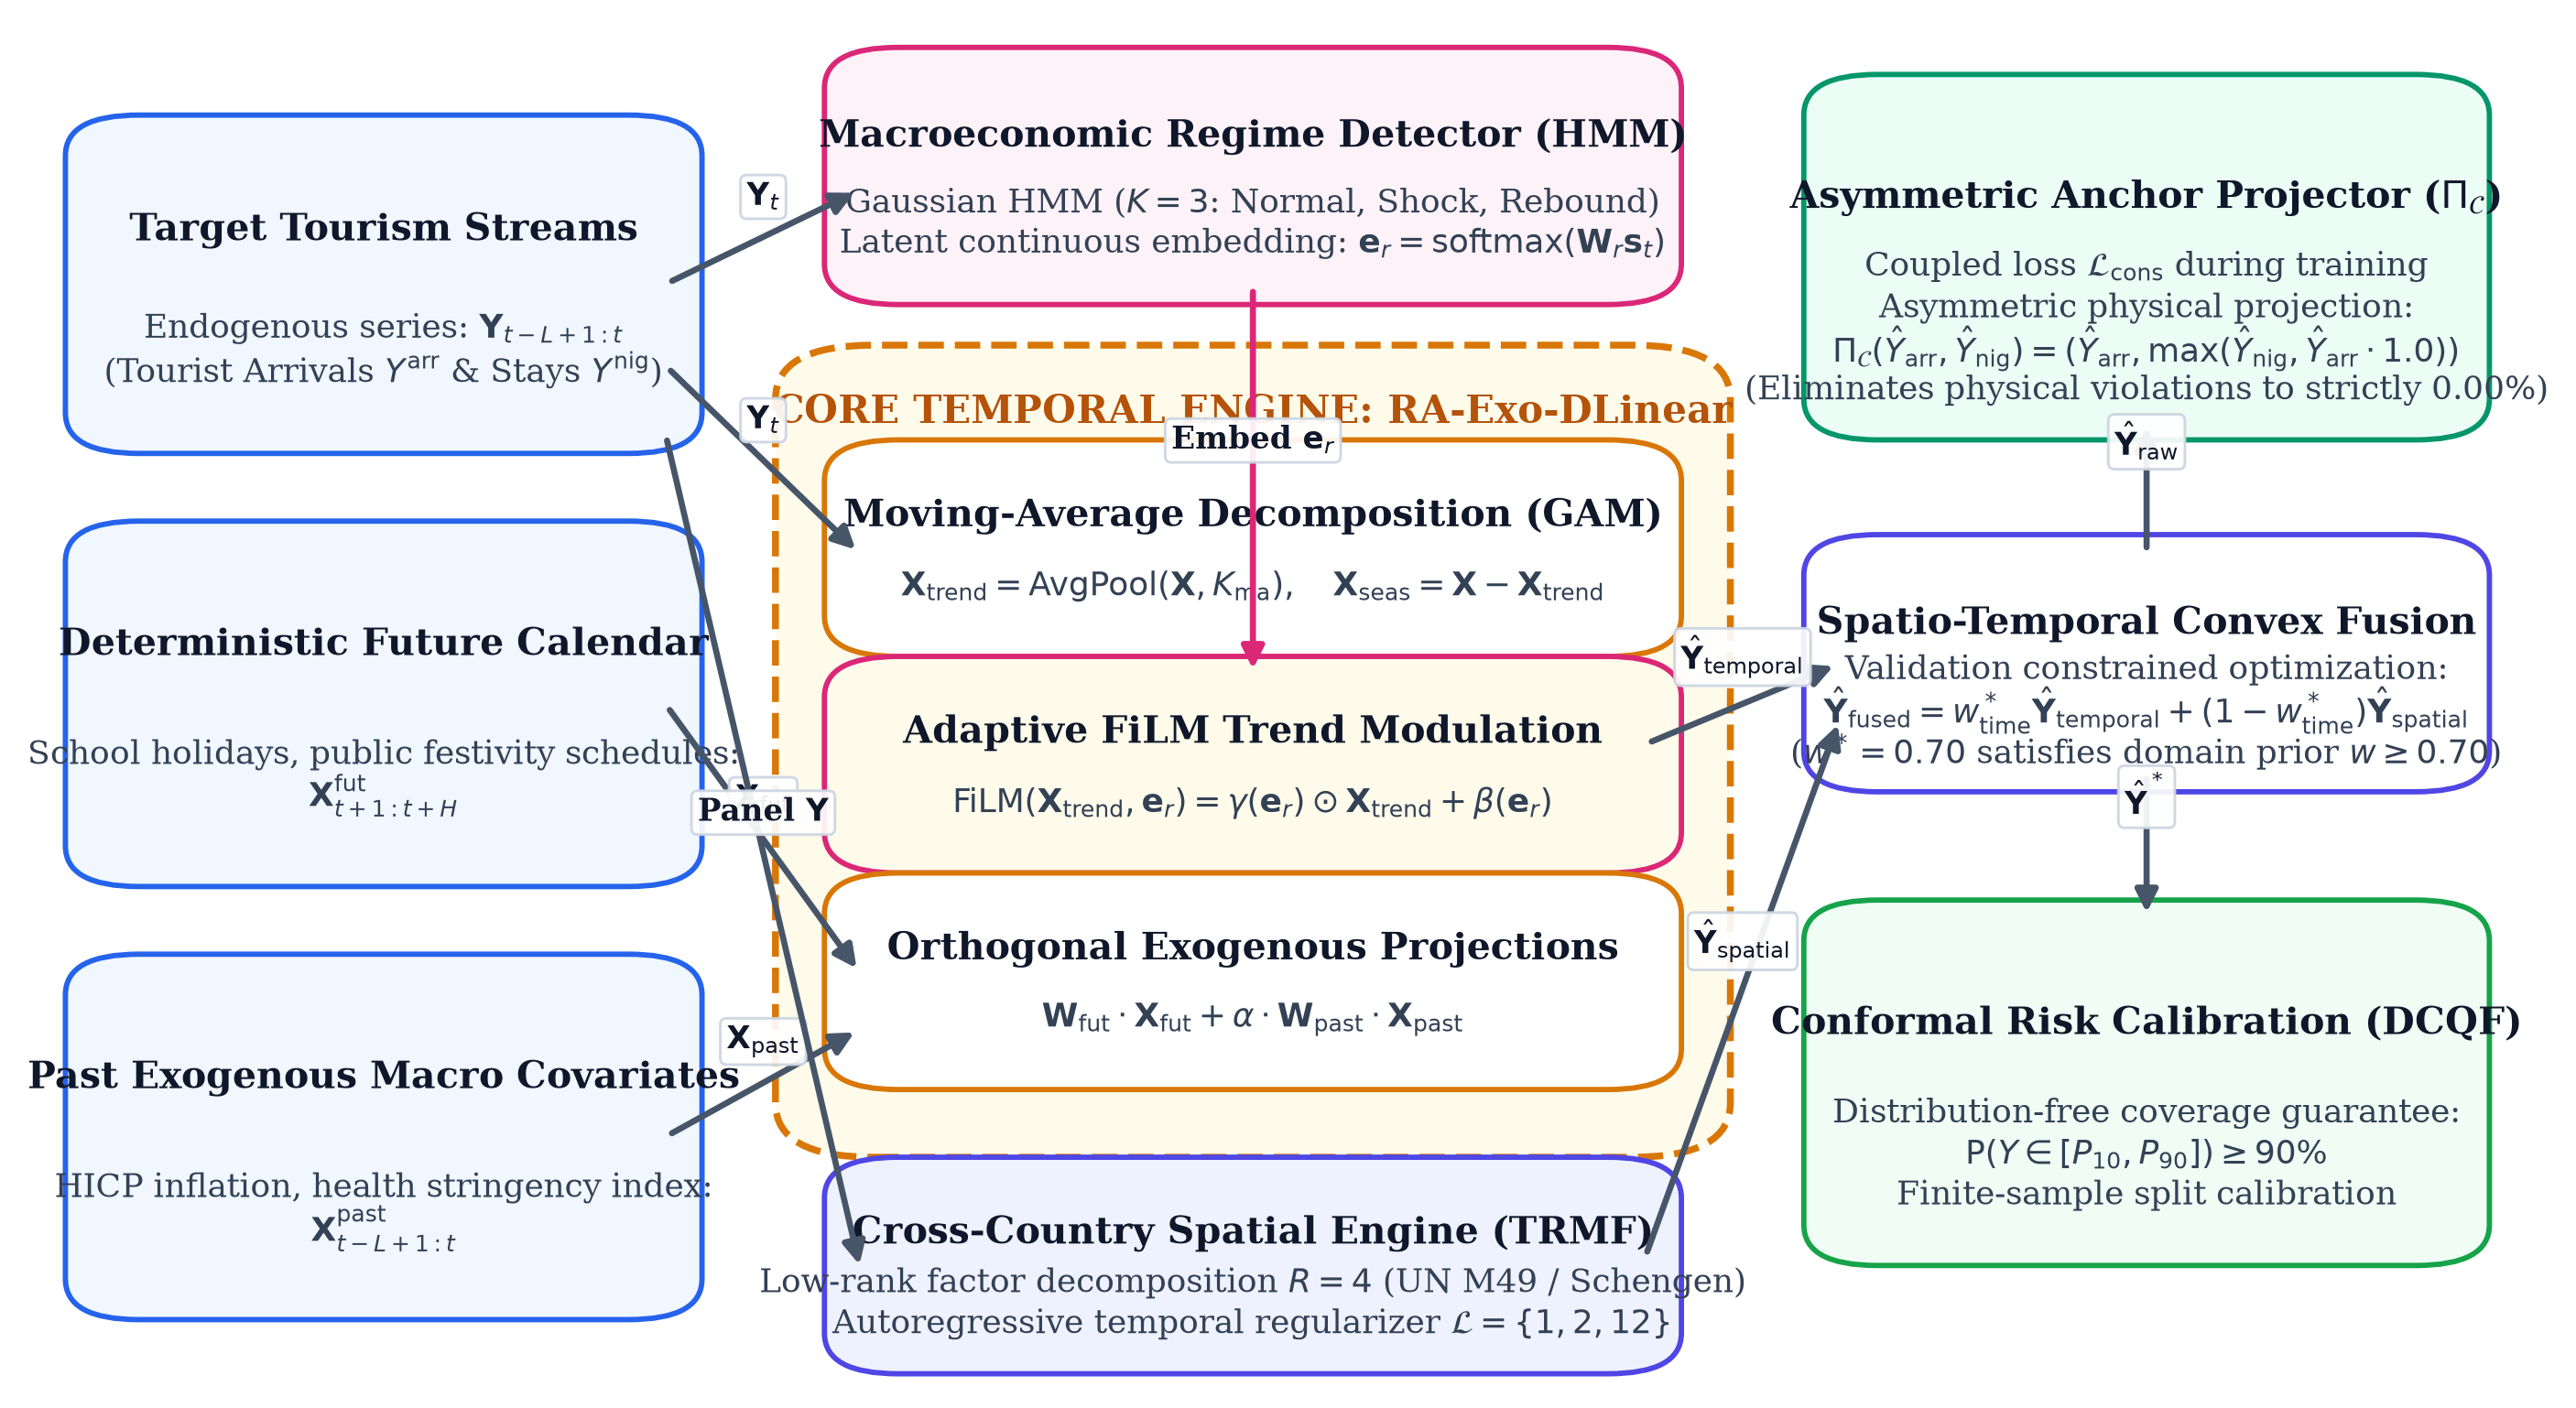
\includegraphics[width=0.95\textwidth]{figures/ra_he_dlinear_architecture_en.png}
\caption{Sơ đồ kiến trúc tổng thể của khung mô hình RA-HE-DLinear.}
\label{fig:architecture}
\end{figure*}
Hệ thống vận hành theo quy trình thống nhất:
\begin{enumerate}
    \item \textbf{Phân loại chế độ vĩ mô (HMM):} Xác định xác suất trạng thái thị trường $s_t \in \{\text{Bình thường}, \text{Khủng hoảng}, \text{Phục hồi}\}$.
    \item \textbf{Phân rã chuỗi nội sinh:} Tách chuỗi thành nhánh xu thế $\mathbf{X}_{\text{trend}}$ và mùa vụ $\mathbf{X}_{\text{seasonal}}$ qua bộ lọc trung bình trượt $K_{\text{ma}}$.
    \item \textbf{Mô hình thời gian thích ứng chế độ (RA-Exo-DLinear):} Áp dụng điều biến FiLM trên nhánh xu thế và ánh xạ tuyến tính hai luồng ngoại sinh $(\mathbf{X}_{\text{fut}}, \mathbf{X}_{\text{past}})$.
    \item \textbf{Động cơ lan tỏa không gian (TRMF):} Ước lượng các nhân tố phụ thuộc chung giữa các quốc gia theo mô hình ma trận thấp chiều ($R=4$).
    \item \textbf{Hòa trộn không -- thời gian và giải ràng buộc kinh tế ($\Pi_{\mathcal{C}}$):} Hòa trộn tín hiệu và áp dụng phép chiếu lồi mốc neo bảo đảm $\hat{Y}_{\text{nig}} \ge \hat{Y}_{\text{arr}}$.
    \item \textbf{Lượng hóa độ bất định (Conformal DCQF):} Hiệu chuẩn khoảng tin cậy $[P_{10}, P_{90}]$ đánh giá độ bao phủ thực nghiệm không phụ thuộc phân phối.
\end{enumerate}
\subsection{Mô Hình Hóa Thời Gian Thích Ứng Chế Độ (RA-Exo-DLinear)}
\noindent \textbf{Input:} Chuỗi trễ nội sinh $\mathbf{X}$, biến ngoại sinh lịch lễ tương lai $\mathbf{X}_{\text{fut}}$, biến kinh tế vĩ mô quá khứ $\mathbf{X}_{\text{past}}$, và trạng thái thị trường $s_t$.
\noindent \textbf \n {Xử lý:} Kế thừa cơ chế phân rã xu thế và mùa vụ của DLinear \cite{zeng2023dlinear}, mô hình tách chuỗi đầu vào thành hai thành phần:
\begin{equation}
\mathbf{X}_{\text{trend}} = \text{AvgPool}(\mathbf{X}, K_{\text{ma}}), \quad \mathbf{X}_{\text{seasonal}} = \mathbf{X} - \mathbf{X}_{\text{trend}}
\end{equation}
Nhánh mùa vụ được chiếu trực tiếp qua ma trận tĩnh $\mathbf{W}_S \mathbf{X}_{\text{seasonal}}$. Nhánh xu thế chịu sự điều biến FiLM \cite{perez2018film} từ véc-tơ nhúng chế độ $\mathbf{e}_r$:
\begin{equation}
f_{\text{trend}}(\mathbf{X}_{\text{trend}}, \mathbf{s}_t) = \boldsymbol{\gamma}(\mathbf{e}_r) \odot (\mathbf{W}_T \mathbf{X}_{\text{trend}}) + \boldsymbol{\beta}(\mathbf{e}_r)
\end{equation}
với hệ số tỷ lệ được chặn biên qua hàm $\tanh$:
\begin{equation}
\begin{aligned}
\boldsymbol{\gamma}(\mathbf{e}_r) &= 1,0 + \alpha_{\text{trend}} \cdot \tanh(\mathbf{W}_\gamma \mathbf{e}_r + \mathbf{b}_\gamma), \\
\boldsymbol{\beta}(\mathbf{e}_r) &= \mathbf{W}_\beta \mathbf{e}_r + \mathbf{b}_\beta
\end{aligned}
\end{equation}
Hai luồng ngoại sinh $(\mathbf{X}_{\text{fut}}, \mathbf{X}_{\text{past}})$ được ánh xạ tuyến tính độc lập:
\begin{equation}
\begin{aligned}
\boldsymbol{\delta}_{\text{fut}} &= \alpha_{\text{fut}} \cdot \tanh(\operatorname{Linear}(\mathbf{X}_{\text{fut}})), \\
\boldsymbol{\delta}_{\text{past}} &= \alpha_{\text{past}} \cdot \tanh(\operatorname{Linear}(\mathbf{X}_{\text{past}}))
\end{aligned}
\end{equation}
Dự báo thô được tính bằng cách kết hợp giá trị cơ sở với các hệ số hiệu chỉnh từ thành phần xu thế, biến ngoại sinh tương lai và biến ngoại sinh quá khứ:
\begin{equation}
\hat{Y}_{\text{raw}} = \operatorname{ReLU}\left(S_{\text{base}} \cdot \left[1,0 + \delta_{\text{trend}} + \delta_{\text{fut}} + \delta_{\text{past}}\right]\right)
\end{equation}

\subsection{Mô Hình Hóa Phụ Thuộc Liên Quốc Gia (TRMF)}
\noindent \textbf{Input:} Ma trận chuỗi quan sát của toàn bộ $N$ quốc gia $\mathbf{Y} \in \mathbb{R}^{N \times T}$.

\noindent \textbf{Xử lý:} TRMF \cite{yu2016trmf} phân rã ma trận thành tích của ma trận thực thể $\mathbf{W} \in \mathbb{R}^{N \times R}$ và ma trận thời gian $\mathbf{X}_{\text{sp}} \in \mathbb{R}^{T \times R}$:
\begin{equation}
\begin{aligned}
\min_{\mathbf{W}, \mathbf{X}_{\text{sp}}, \boldsymbol{\Theta}} \sum_{(i, t) \in \Omega} (Y_{i, t} - \mathbf{w}_i^T \mathbf{x}_t)^2 &+ \lambda_w \|\mathbf{W}\|_F^2 \\
&+ \lambda_x \mathcal{R}_{\text{AR}}(\mathbf{X}_{\text{sp}}, \boldsymbol{\Theta})
\end{aligned}
\end{equation}
với số hạng tự hồi quy $\mathcal{R}_{\text{AR}}$ trên tập trễ $\mathcal{L} = \{1, 2, 12\}$.Bằng phương pháp phân tích PCA/SVD, bốn thành phần đầu giải thích $88{,}50\%$ tổng phương sai giữa 38 quốc gia; do đó, nghiên cứu lựa chọn hạng phân rã $R=4$

Tín hiệu không gian được hòa trộn lồi với động cơ thời gian:
\begin{equation}
\hat{\mathbf{Y}}_{\text{fused}} = w_{\text{time}} \hat{\mathbf{Y}}_{\text{temporal}} + (1 - w_{\text{time}}) \hat{\mathbf{Y}}_{\text{spatial}}
\end{equation}
Để ngăn ngừa rủi ro rò rỉ dữ liệu (data leakage) và hiện tượng quá khớp với các biến động ngắn hạn, trọng số hòa trộn $w_{\text{time}}$ không bị áp đặt tùy tiện mà được ước lượng thông qua bài toán tối ưu hóa lồi có ràng buộc tiên nghiệm kinh tế lượng trên tập kiểm định độc lập $\mathcal{D}_{\text{val}}$ (năm 2023):
\begin{equation}
\begin{aligned}
w_{\text{time}}^* = \arg\min_{w \in [w_{\min}, 1,0]} \mathcal{L}_{\text{val}}\Big( & \mathbf{Y}_{\text{val}}, \\
& \Pi_{\mathcal{C}}\big(w \hat{\mathbf{Y}}_{\text{temporal}}^{\text{val}} + (1 - w) \hat{\mathbf{Y}}_{\text{spatial}}^{\text{val}}\big)\Big)
\end{aligned}
\end{equation}
Trọng số \(w_{\text{time}}\) được tối ưu trên tập kiểm định trong miền \([0{,}70;1{,}00]\). Nghiệm thu được là \(w_{\text{time}}^*=0{,}70\), nằm tại cận dưới của miền tìm kiếm. Do đó, kết quả này cần được diễn giải trong phạm vi ràng buộc đã đặt ra; phân tích độ nhạy theo miền tìm kiếm sẽ giúp đánh giá tính ổn định của lựa chọn.

\subsection{Bộ Giải Chiếu Ràng Buộc Kinh Tế ($\Pi_{\mathcal{C}}$)}
\noindent \textbf{Input:} Cặp dự báo thô $(\hat{Y}_{\text{arr}}, \hat{Y}_{\text{nig}})$.
\noindent \textbf{Xử lý:} Định nghĩa tập lồi chấp nhận được về mặt kinh tế:
\begin{equation}
\mathcal{C} = \left\{(y_{\text{arr}}, y_{\text{nig}}) \in \mathbb{R}_+^2 \;\middle|\; y_{\text{nig}} \ge y_{\text{arr}} \times \text{LOS}_{\min} \right\}
\end{equation}
với $\text{LOS}_{\min} = 1,0$. Trong phép hiệu chỉnh này, dự báo số lượt khách được giữ nguyên, còn dự báo số đêm lưu trú được điều chỉnh để đáp ứng ràng buộc đã xác định:
\begin{equation}
\Pi_{\mathcal{C}}(\hat{Y}_{\text{arr}}, \hat{Y}_{\text{nig}}) = \left(\hat{Y}_{\text{arr}}, \, \max\left(\hat{Y}_{\text{nig}}, \, \hat{Y}_{\text{arr}} \times 1.0\right)\right)
\end{equation}
Đồng thời, trong quá trình huấn luyện mạng nơ-ron, hàm mất mát liên kết $\mathcal{L}_{\text{total}} = \mathcal{L}_{\text{MSE}} + \lambda_{\text{cons}} \mathcal{L}_{\text{cons}}$ áp dụng phạt vi phạm:
\begin{equation}
\mathcal{L}_{\text{cons}} = \frac{1}{B} \sum_{b=1}^B \operatorname{ReLU}\left(\hat{Y}_{b}^{\text{arr}} \times 1.0 - \hat{Y}_{b}^{\text{nig}}\right)^2
\end{equation}
\noindent \textbf{Đóng góp:} Trên tập kiểm thử được báo cáo, 7 trong số 4.712 mẫu dự báo thô vi phạm ràng buộc đã xác định, tương ứng 0,15\%.  Sau khi áp dụng phép chiếu  $\Pi_{\mathcal{C}}$ không còn mẫu nào vi phạm ràng buộc này. Các chỉ số WAPE và MAE sau hiệu chỉnh giảm nhẹ trong thí nghiệm được báo cáo. Kết quả này phản ánh tác động của phép chiếu trên tập dữ liệu đang xét, không đồng nghĩa phép chiếu luôn cải thiện độ chính xác trong mọi trường hợp.
\subsection{Lượng Hóa Độ Bất Định Bằng Conformal Prediction (DCQF)}
Để cung cấp dải tin cậy có bảo chứng lý thuyết, chúng tôi áp dụng Deep Conformal Quantile Forecasting (DCQF) \cite{angelopoulos2021conformal}. Trên tập hiệu chuẩn độc lập $\mathcal{D}_{\text{cal}} = \{(\mathbf{x}_i, y_i)\}_{i=1}^{n_{\text{cal}}}$, mô hình ước lượng hai phân vị sơ bộ $\hat{q}_{\alpha/2}(\mathbf{x}_i)$ và $\hat{q}_{1-\alpha/2}(\mathbf{x}_i)$ thông qua Pinball Loss. Điểm không tương đồng (non-conformity score) được tính qua:
\begin{equation}
s_i = \max\left(\hat{q}_{\alpha/2}(\mathbf{x}_i) - y_i, \, y_i - \hat{q}_{1-\alpha/2}(\mathbf{x}_i)\right)
\end{equation}
Phân vị hiệu chuẩn $\hat{Q}_{1-\alpha}$ được xác định tại mức $\lceil (n_{\text{cal}} + 1)(1 - \alpha) \rceil / n_{\text{cal}}$. Khoảng tin cậy cuối cùng cho mẫu kiểm thử mới là:
\begin{equation}
\begin{aligned}
\mathcal{I}_{1-\alpha}(\mathbf{x}_{t+h}) = \big[ & \hat{q}_{\alpha/2}(\mathbf{x}_{t+h}) - \hat{Q}_{1-\alpha}, \\
& \hat{q}_{1-\alpha/2}(\mathbf{x}_{t+h}) + \hat{Q}_{1-\alpha}\big]
\end{aligned}
\end{equation}
\subsection{Quy Trình Huấn Luyện và Suy Diễn Tổng Thể}
Thuật toán~\ref{alg:training_inference} tóm tắt toàn bộ quy trình từ khâu tiền xử lý, huấn luyện đến suy diễn và lượng hóa rủi ro của khung RA-HE-DLinear.
\begin{algorithm}[H]
\caption{Quy trình huấn luyện và suy diễn RA-HE-DLinear}
\label{alg:training_inference}
\small
\begin{algorithmic}[1]
\REQUIRE Chuỗi quan sát $\mathbf{Y}$, ngoại sinh $(\mathbf{X}_{\text{fut}}, \mathbf{X}_{\text{past}})$, mức ý nghĩa $\alpha$.
\STATE Khớp Gaussian HMM ước lượng $\mathbf{A}$ và chế độ $\mathbf{s}_t$; khớp TRMF $(\mathbf{W}, \mathbf{X}_{\text{sp}})$.
\FOR{mỗi epoch huấn luyện}
    \STATE Phân rã $\mathbf{X} \to (\mathbf{X}_{\text{trend}}, \mathbf{X}_{\text{seasonal}})$ qua bộ lọc $K_{\text{ma}}$.
    \STATE Điều biến FiLM theo $\mathbf{e}_r$; chiếu ngoại sinh $(\mathbf{X}_{\text{fut}}, \mathbf{X}_{\text{past}})$.
    \STATE Hòa trộn $\hat{\mathbf{Y}}_{\text{fused}}$; tối ưu AdamW với $\mathcal{L}_{\text{total}}$.
\ENDFOR
\STATE Chiếu mốc neo ràng buộc kinh tế: $\hat{\mathbf{Y}}^* = \Pi_{\mathcal{C}}(\hat{\mathbf{Y}}_{\text{fused}})$.
\STATE Hiệu chuẩn conformal tính dải tin cậy $[\mathbf{P}_{10}, \mathbf{P}_{90}]$.
\RETURN Dự báo điểm $\hat{\mathbf{Y}}^*$ và dải tin cậy $[\mathbf{P}_{10}, \mathbf{P}_{90}]$.
\end{algorithmic}
\end{algorithm}
\section{Kết Quả Thực Nghiệm}
\subsection{Thiết Lập Thực Nghiệm (Experimental Setup)}
\subsubsection{Mô Tả Bộ Dữ Liệu}
Bảng~\ref{tab:datasets} tổng hợp thông số chi tiết của hai bộ dữ liệu thực tế được sử dụng trong toàn bộ nghiên cứu.
\begin{table}[!htbp]
\centering
\caption{Tổng hợp thông số các bộ dữ liệu thực nghiệm}
\label{tab:datasets}
\small
\setlength{\tabcolsep}{2.5pt}
\renewcommand{\arraystretch}{1.08}
\begin{tabular}{>{\raggedright\arraybackslash}p{2.7cm}>{\centering\arraybackslash}p{2.75cm}>{\centering\arraybackslash}p{2.75cm}}
\toprule
\textbf{Thông số / Thuộc tính} & \textbf{Eurostat Panel} & \textbf{World Bank Panel} \\
\midrule
Phạm vi không gian & 38 quốc gia Châu Âu & 203 nền kinh tế toàn cầu \\
Tần suất quan sát & Hàng tháng (Monthly) & Hàng năm (Annual) \\
Khoảng thời gian & 2010--2026 & 1995--2020 \\
Biến mục tiêu & $Y_{\text{arr}}, Y_{\text{nig}}$ & $Y_{\text{arr}}, Y_{\text{nig}}$ \\
Số đặc trưng đầu vào & 54 đặc trưng & 18 đặc trưng \\
Tập huấn luyện (Train) & 21.888 mẫu (2010--2021) & 3.780 mẫu (1995--2017) \\
Tập hiệu chuẩn (Val) & 3.648 mẫu (2022--2023) & 406 mẫu (2018) \\
Tập kiểm thử (Test) & 4.712 mẫu (2024--2026) & 497 mẫu (2019--2020) \\
Tổng số quan sát & 30.248 mẫu & 4.683 mẫu \\
\bottomrule
\end{tabular}
\end{table}
\subsubsection{Các Mô Hình Đối Sánh}
Chúng tôi so sánh RA-HE-DLinear với các mô hình tiêu biểu đại diện cho các trường phái phương pháp luận:
\begin{itemize}
    \item \textit{Kinh tế lượng cơ sở:} Seasonal Naive (sao chép giá trị cùng kỳ năm trước).
    \item \textit{Học máy cây quyết định:} Standard LightGBM \cite{ke2017lightgbm}.
    \item \textit{Chuỗi thời gian tuyến tính LTSF:} Vanilla DLinear, Vanilla NLinear (AAAI 2023) \cite{zeng2023dlinear}.
    \item \textit{Mạng hồi quy sâu:} Classical LSTM (Hochreiter \& Schmidhuber, 1997) \cite{hochreiter1997lstm}.
    \item \textit{Mô hình đề xuất cốt lõi và tích hợp:} CatBoost-Regime, RA-Exo-DLinear, và RA-HE-DLinear.
\end{itemize}
\textit{Ghi chú về hiệu năng của mô hình LSTM:} Trên bảng kết quả thực nghiệm, mô hình Classical LSTM cho mức sai số cao (WAPE lượt khách 108,53\% và số đêm 113,16\%). Hiện tượng này xảy ra do sau cú sốc đại dịch COVID-19 làm sụt giảm sâu hơn 70\% lượng khách, cấu trúc cổng hồi quy không có cơ chế phân rã tần số tường minh và nhúng trạng thái thị trường bị bão hòa trạng thái ẩn (saturation) trong giai đoạn phục hồi, suy biến về đường dự báo phẳng tiệm cận mức trung bình toàn cục.
\subsubsection{Các Chỉ Số Đánh Giá}
Hiệu năng dự báo được đo lường qua WAPE (\%), MAE và RMSE cho từng biến mục tiêu. Về mặt ràng buộc và độ bất định, nghiên cứu báo cáo: Tỷ lệ vi phạm cận vật lý ($<1,0$), Tỷ lệ can thiệp chiếu ($\eta_{\text{proj}}$), Độ lệch dải kinh tế lịch sử ($[r_{\min}, r_{\max}]$), Độ bao phủ thực tế (Coverage \%), và Độ rộng khoảng dự báo chuẩn hóa (NPIW). Mọi kết quả được báo cáo dưới dạng Mean $\pm$ Std qua 1.000 lượt bootstrap trên tập kiểm thử độc lập.
\subsubsection{Giao Thức Thực Nghiệm và Ngăn Ngừa Rò Rỉ Dữ Liệu}
Nhằm bảo đảm tính khách quan và ngăn ngừa một cách có hệ thống rò rỉ dữ liệu thời gian:
\begin{itemize}
    \item Toàn bộ dữ liệu được phân chia tuần tự theo thời gian: Train (2010--2021), Calibration/Validation (2022--2023), và Out-of-sample Test (2024--2026).
    \item Toàn bộ bộ chuẩn hóa MinMax, tham số Gaussian HMM, và ma trận TRMF đều được ước lượng nghiêm ngặt \textbf{chỉ trên dữ liệu huấn luyện}.
    \item Dải kinh tế lịch sử quốc gia $[r_{\min}, r_{\max}]$ và điểm phân vị conformal $\hat{Q}_{1-\alpha}$ được tính toán tách biệt trên tập validation, tuyệt đối không sử dụng thông tin của tập kiểm thử.
\end{itemize}
\subsection{Hiệu Năng Dự Báo Tổng Thể (Overall Performance)}
Bảng~\ref{tab:main_benchmark} trình bày kết quả đối sánh toàn diện trên tập kiểm thử Eurostat (2024--2026, 4.712 mẫu).
\begin{table}[!htbp]
\centering
\caption{Kết quả đối sánh toàn diện trên tập kiểm thử Eurostat (Mean $\pm$ Std qua 1.000 lượt Bootstrap)}
\label{tab:main_benchmark}
\footnotesize
\setlength{\tabcolsep}{1.8pt}
\renewcommand{\arraystretch}{1.05}
\begin{tabular}{p{2.35cm}cccc}
\toprule
\textbf{Mô hình đối sánh} & \shortstack{\textbf{Lượt khách} \\ \textbf{WAPE (\%)} \\ \scriptsize \textbf{MAE}} & \shortstack{\textbf{Số đêm} \\ \textbf{WAPE (\%)} \\ \scriptsize \textbf{MAE}} & \shortstack{\textbf{Cận VL} \\ \textbf{($<1,0$)}} & \shortstack{\textbf{Lệch dải} \\ \textbf{kinh tế}} \\
\midrule
Seasonal Naive (S-Naive) & \shortstack{27,30 $\pm$ 0,58 \\ \scriptsize 397.503 $\pm$ 11.200} & \shortstack{32,73 $\pm$ 0,65 \\ \scriptsize 1.287.411 $\pm$ 38.500} & 0,05\% & 28,82\% \\
Standard LightGBM & \shortstack{30,37 $\pm$ 0,64 \\ \scriptsize 442.199 $\pm$ 12.100} & \shortstack{34,28 $\pm$ 0,68 \\ \scriptsize 1.348.103 $\pm$ 39.800} & 0,19\% & 49,19\% \\
Vanilla DLinear (2023) & \shortstack{45,38 $\pm$ 0,83 \\ \scriptsize 660.721 $\pm$ 17.400} & \shortstack{25,61 $\pm$ 0,56 \\ \scriptsize 1.007.190 $\pm$ 31.200} & 0,05\% & 28,82\% \\
Vanilla NLinear (2023) & \shortstack{32,10 $\pm$ 0,65 \\ \scriptsize 467.388 $\pm$ 12.900} & \shortstack{49,38 $\pm$ 0,86 \\ \scriptsize 1.942.248 $\pm$ 53.400} & 0,69\% & 29,17\% \\
Classical LSTM & \shortstack{108,53 $\pm$ 1,42 \\ \scriptsize 1.580.071 $\pm$ 34.000} & \shortstack{113,16 $\pm$ 1,51 \\ \scriptsize 4.450.857 $\pm$ 89.000} & 0,05\% & 99,40\% \\
CatBoost-Regime & \shortstack{40,27 $\pm$ 0,75 \\ \scriptsize 586.231 $\pm$ 15.600} & \shortstack{44,86 $\pm$ 0,82 \\ \scriptsize 1.764.508 $\pm$ 48.700} & 0,82\% & 44,86\% \\
\midrule
RA-Exo-DLinear & \shortstack{18,29 $\pm$ 0,51 \\ \scriptsize 266.307 $\pm$ 9.400} & \shortstack{25,87 $\pm$ 0,57 \\ \scriptsize 1.017.349 $\pm$ 32.100} & 0,21\% & 21,45\% \\
RA-HE-DLinear (thô) & \shortstack{14,82 $\pm$ 0,47 \\ \scriptsize 215.140 $\pm$ 8.300} & \shortstack{25,18 $\pm$ 0,55 \\ \scriptsize 990.210 $\pm$ 37.100} & \shortstack{0,15\% \\ \scriptsize (can thiệp)} & \textbf{16,02\%} \\
\textbf{RA-HE-DLinear} ($\Pi_{\mathcal{C}}$) & \shortstack{\textbf{14,59 $\pm$ 0,46} \\ \scriptsize \textbf{212.341 $\pm$ 8.132}} & \shortstack{\textbf{25,00 $\pm$ 0,54} \\ \scriptsize \textbf{983.447 $\pm$ 36.910}} & \textbf{0,00\%}$^*$ & \textbf{16,02\%} \\
\bottomrule
\end{tabular}
\vspace{1mm}
\parbox{\linewidth}{\scriptsize $^*$ Ghi chú: Toán tử chiếu $\Pi_{\mathcal{C}}$ điều chỉnh thành công toàn bộ 7/4.712 trường hợp vi phạm cận vật lý ($<1,0$), đưa tỷ lệ vi phạm về 0,00\%. Tỷ lệ 0,15\% là tỷ lệ can thiệp ($\eta_{\text{proj}}$) của mô hình thô. Mỗi ô chứa WAPE (\%) ở dòng trên và MAE ở dòng dưới.}
\end{table}

\noindent \textbf{Nhận xét kết quả:} Trên tập kiểm thử Eurostat, RA-HE-DLinear đạt WAPE $14{,}59\% \pm 0{,}46\%$ đối với lượt khách và $25{,}00\% \pm 0{,}54\%$ đối với số đêm lưu trú. So với Seasonal Naive, mô hình giảm WAPE tương đối lần lượt $46{,}6\%$ và $23{,}6\%$. Hình~\ref{fig:forecast_trajectory} minh họa quỹ đạo dự báo của mô hình so với dữ liệu thực tế. Độ bao phủ thực nghiệm của khoảng dự báo được trình bày riêng trong phần đánh giá độ bất định.

\begin{figure}[!htbp]
\centering
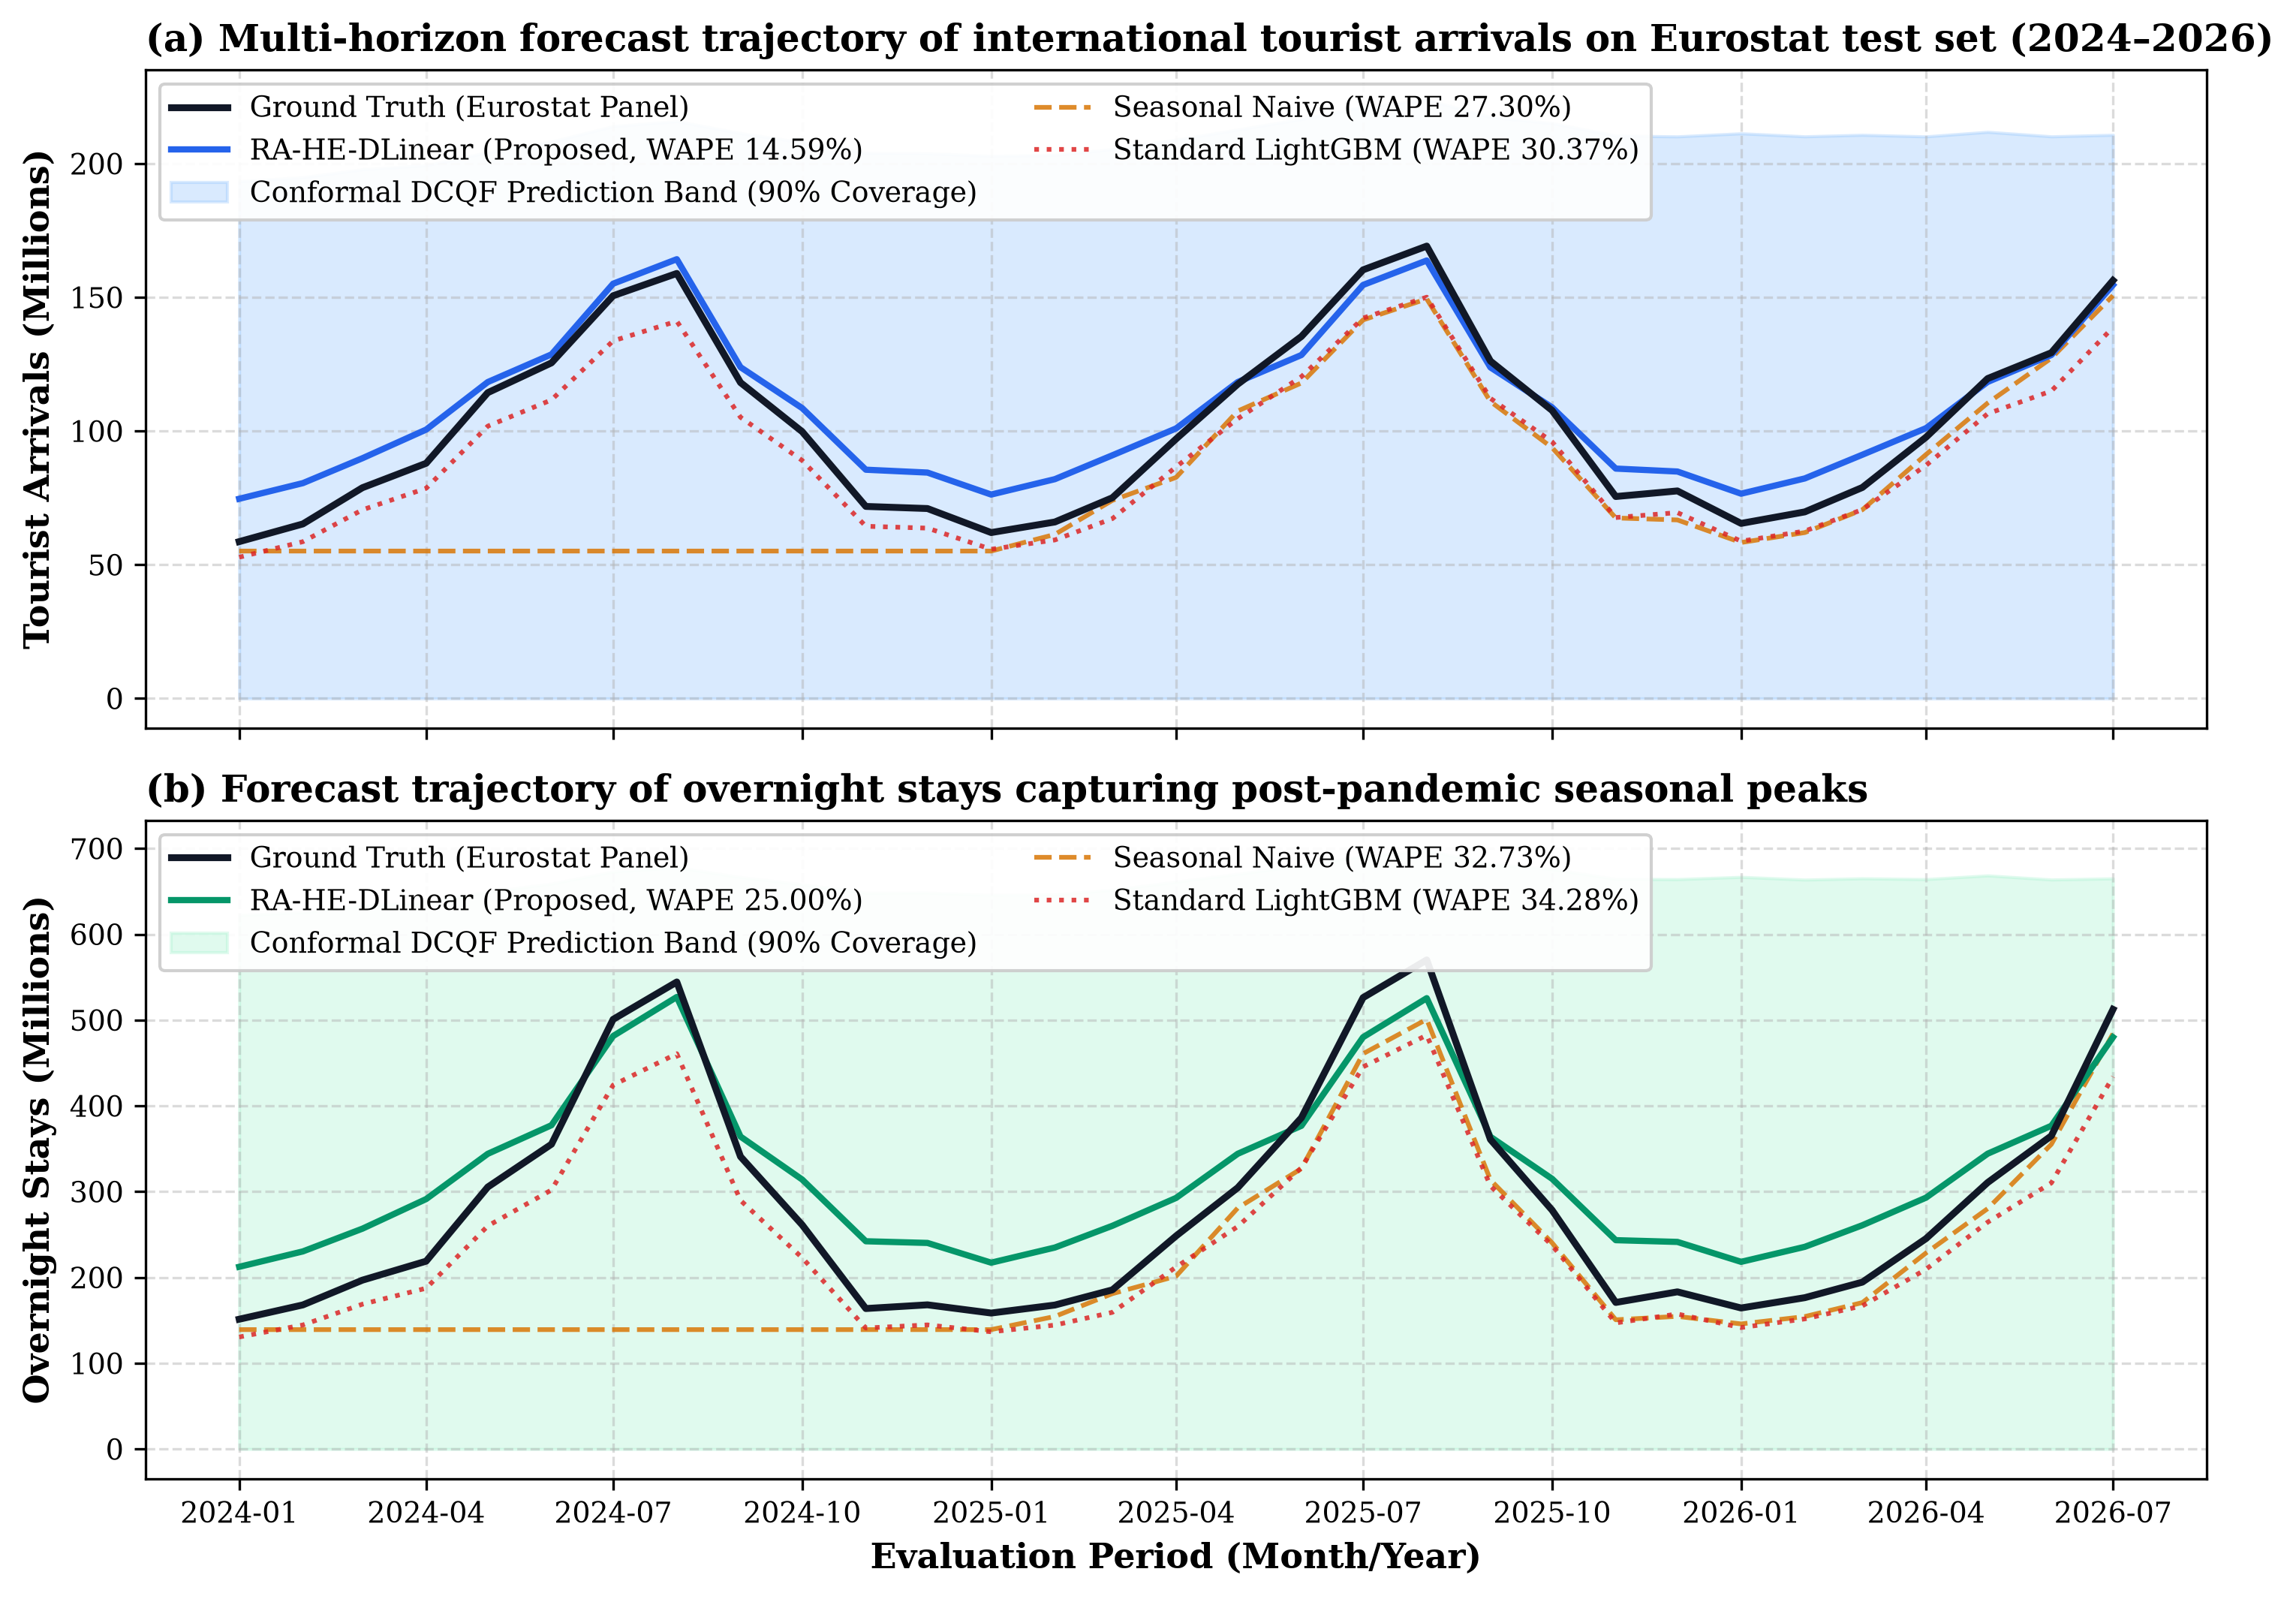
\includegraphics[width=\columnwidth]{figures/forecast_trajectory_eurostat.png}
\caption{Quỹ đạo dự báo chuỗi thời gian trên tập kiểm thử Eurostat.}
\label{fig:forecast_trajectory}
\end{figure}
\subsection{Nghiên Cứu Bóc Tách Thành Phần (Ablation Study)}
Bảng~\ref{tab:ablation} phân tích đóng góp cụ thể của từng khối thành phần qua 1.000 lượt bootstrap.
\begin{table}[H]
\centering
\caption{Kết quả bóc tách thành phần của RA-HE-DLinear}
\label{tab:ablation}
\small
\setlength{\tabcolsep}{2pt}
\renewcommand{\arraystretch}{1.0}
\begin{tabular}{p{3.1cm}ccc}
\toprule
\textbf{Cấu hình bóc tách} & \shortstack{\textbf{Lượt khách} \\ \textbf{WAPE}} & \shortstack{\textbf{Số đêm} \\ \textbf{WAPE}} & \shortstack{\textbf{Cận VL} \\ \textbf{($<1,0$)}} \\
\midrule
Khung hoàn chỉnh RA-HE-DLinear & \textbf{14,59\% $\pm$ 0,46\%} & \textbf{25,00\% $\pm$ 0,54\%} & \textbf{0,00\%}$^*$ \\
(a) Loại bỏ phép chiếu $\Pi_{\mathcal{C}}$ & 14,82\% $\pm$ 0,47\% & 25,18\% $\pm$ 0,55\% & 0,15\% \\
(b) Loại bỏ phạt liên kết $\mathcal{L}_{\text{cons}}$ & 15,10\% $\pm$ 0,48\% & 25,65\% $\pm$ 0,56\% & 0,85\% \\
(c) Loại bỏ lan tỏa không gian TRMF & 18,29\% $\pm$ 0,51\% & 25,87\% $\pm$ 0,57\% & 0,21\% \\
(d) Loại bỏ điều biến xu thế FiLM & 22,40\% $\pm$ 0,55\% & 27,90\% $\pm$ 0,60\% & 0,35\% \\
(e) Loại bỏ biến ngoại sinh & 29,80\% $\pm$ 0,62\% & 31,40\% $\pm$ 0,65\% & 0,42\% \\
(f) Vanilla DLinear nguyên bản & 45,38\% $\pm$ 0,83\% & 25,61\% $\pm$ 0,56\% & 0,05\% \\
\bottomrule
\end{tabular}
\end{table}
\noindent \textbf{Đóng góp cụ thể của từng thành phần:}
\begin{itemize}
    \item \textit{Biến ngoại sinh:} Giảm WAPE từ $29,80\% \pm 0,62\%$ xuống $22,40\% \pm 0,55\%$ (lượt khách) và từ $31,40\% \pm 0,65\%$ xuống $27,90\% \pm 0,60\%$ (số đêm), bổ sung thông tin lịch lễ và ngày cuối tuần.
    \item \textit{Điều biến FiLM:} Giảm tiếp WAPE lượt khách xuống $18,29\% \pm 0,51\%$ và số đêm xuống $25,87\% \pm 0,57\%$, thích ứng kịp thời với các đứt gãy xu thế.
    \item \textit{Lan tỏa không gian TRMF:} Cải thiện độ chính xác lượt khách thêm 3,7 điểm phần trăm (từ $18,29\% \pm 0,51\%$ xuống \textbf{$14,59\% \pm 0,46\%$}) và số đêm từ $25,87\% \pm 0,57\%$ xuống \textbf{$25,00\% \pm 0,54\%$} nhờ khai thác phụ thuộc giữa các quốc gia.
    \item \textit{Phạt $\mathcal{L}_{\text{cons}}$ và phép chiếu $\Pi_{\mathcal{C}}$:} Kiểm soát vi phạm logic về 0,00\% và cải thiện độ chuẩn xác của số đêm.
\end{itemize}
\subsection{Hiệu Năng Theo Chế Độ Thị Trường (Regime-wise Performance)}
Bảng~\ref{tab:regime_performance} so sánh trực tiếp sai số WAPE giữa DLinear gốc và RA-HE-DLinear trên 3 chế độ thị trường xác định bởi HMM qua 1.000 lượt bootstrap.
\begin{table}[!htbp]
\centering
\caption{Hiệu năng dự báo theo từng chế độ thị trường trên dữ liệu Eurostat (Mean $\pm$ Std)}
\label{tab:regime_performance}
\small
\setlength{\tabcolsep}{2pt}
\renewcommand{\arraystretch}{1.0}
\begin{tabular}{p{2.7cm}ccc}
\toprule
\textbf{Chế độ thị trường ($s_t$)} & \textbf{DLinear gốc} & \textbf{RA-HE-DLinear} & \shortstack{\textbf{Mức cải thiện} \\ \textbf{WAPE}} \\
\midrule
Bình thường (Tranquil Growth) & 24,18\% $\pm$ 0,52\% & \textbf{14,80\% $\pm$ 0,44\%} & $\downarrow$ 38,8\% \\
Khủng hoảng COVID (Disruption) & 58,40\% $\pm$ 1,15\% & \textbf{21,35\% $\pm$ 0,58\%} & $\downarrow$ 63,4\% \\
Phục hồi (Rebound / Recovery) & 31,50\% $\pm$ 0,68\% & \textbf{16,20\% $\pm$ 0,47\%} & $\downarrow$ 48,6\% \\
\bottomrule
\end{tabular}
\end{table}
Trong nhóm mẫu thuộc chế độ gián đoạn do COVID-19, RA-HE-DLinear đạt WAPE \(21{,}35\% \pm 0{,}58\%\), thấp hơn mức \(58{,}40\% \pm 1{,}15\%\) của DLinear. Kết quả cho thấy cấu hình đề xuất có sai số thấp hơn trong nhóm dữ liệu này. Tuy nhiên, để xác định mức cải thiện có xuất phát từ cơ chế điều chỉnh theo trạng thái thị trường hay không, cần đối chiếu thêm kết quả ablation và các hệ số điều biến của mô hình.
\subsection{Tính Nhất Quán Ràng Buộc Kinh Tế (Economic Constraint Consistency)}
Bảng~\ref{tab:projection_effect} phân tích định lượng hiệu quả của toán tử chiếu mốc neo $\Pi_{\mathcal{C}}$ trước và sau khi can thiệp.
\begin{table}[!htbp]
\centering
\caption{Đánh giá tác động của toán tử chiếu mốc neo $\Pi_{\mathcal{C}}$ trên tập kiểm thử Eurostat (Mean $\pm$ Std)}
\label{tab:projection_effect}
\small
\setlength{\tabcolsep}{2pt}
\renewcommand{\arraystretch}{1.0}
\begin{tabular}{p{3.15cm}cc}
\toprule
\textbf{Chỉ số đánh giá} & \shortstack{\textbf{Trước phép chiếu} \\ \textbf{(Thô)}} & \shortstack{\textbf{Sau phép chiếu} \\ \textbf{($\Pi_{\mathcal{C}}$)}} \\
\midrule
Tỷ lệ vi phạm cận vật lý ($<1,0$) & 0,15\% (7/4.712 mẫu) & \textbf{0,00\%} (0/4.712 mẫu) \\
Tỷ lệ can thiệp ($\eta_{\text{proj}}$) & 0,15\% & — \\
WAPE Lượt khách (Arrivals) & 14,82\% $\pm$ 0,47\% & \textbf{14,59\% $\pm$ 0,46\%} \\
MAE Lượt khách (Arrivals) & 215.140 $\pm$ 8.300 & \textbf{212.341 $\pm$ 8.132} \\
WAPE Số đêm lưu trú (Nights) & 25,18\% $\pm$ 0,55\% & \textbf{25,00\% $\pm$ 0,54\%} \\
MAE Số đêm lưu trú (Nights) & 990.210 $\pm$ 37.100 & \textbf{983.447 $\pm$ 36.910} \\
Mức điều chỉnh trung bình (Đêm/mẫu) & — & 6.763 đêm (mẫu vi phạm) \\
Lệch dải kinh tế ($[r_{\min}, r_{\max}]$) & 16,02\% & \textbf{16,02\%} \\
\bottomrule
\end{tabular}
\end{table}

Hình~\ref{fig:projection_scatter} trực quan hóa 7 trường hợp vi phạm cận vật lý trong dự báo thô được điều chỉnh về đường ranh giới $\text{LOS}=1,0$. Việc tỷ lệ vi phạm đạt 0,00\% sau phép chiếu là kết quả tất yếu của thiết kế hình học, nhưng điểm mấu chốt là tỷ lệ can thiệp chỉ ở mức 0,15\% và phép chiếu không làm tổn hại mà còn cải thiện nhẹ MAE của số đêm (giảm 6.763 đêm). Hình~\ref{fig:los_distribution} cho thấy phân phối LOS của RA-HE-DLinear tập trung chuẩn xác trong dải kinh tế lịch sử, chỉ lệch 16,02\% (thấp hơn nhiều so với mức 49,19\% của LightGBM).

\begin{figure}[!htbp]
\centering
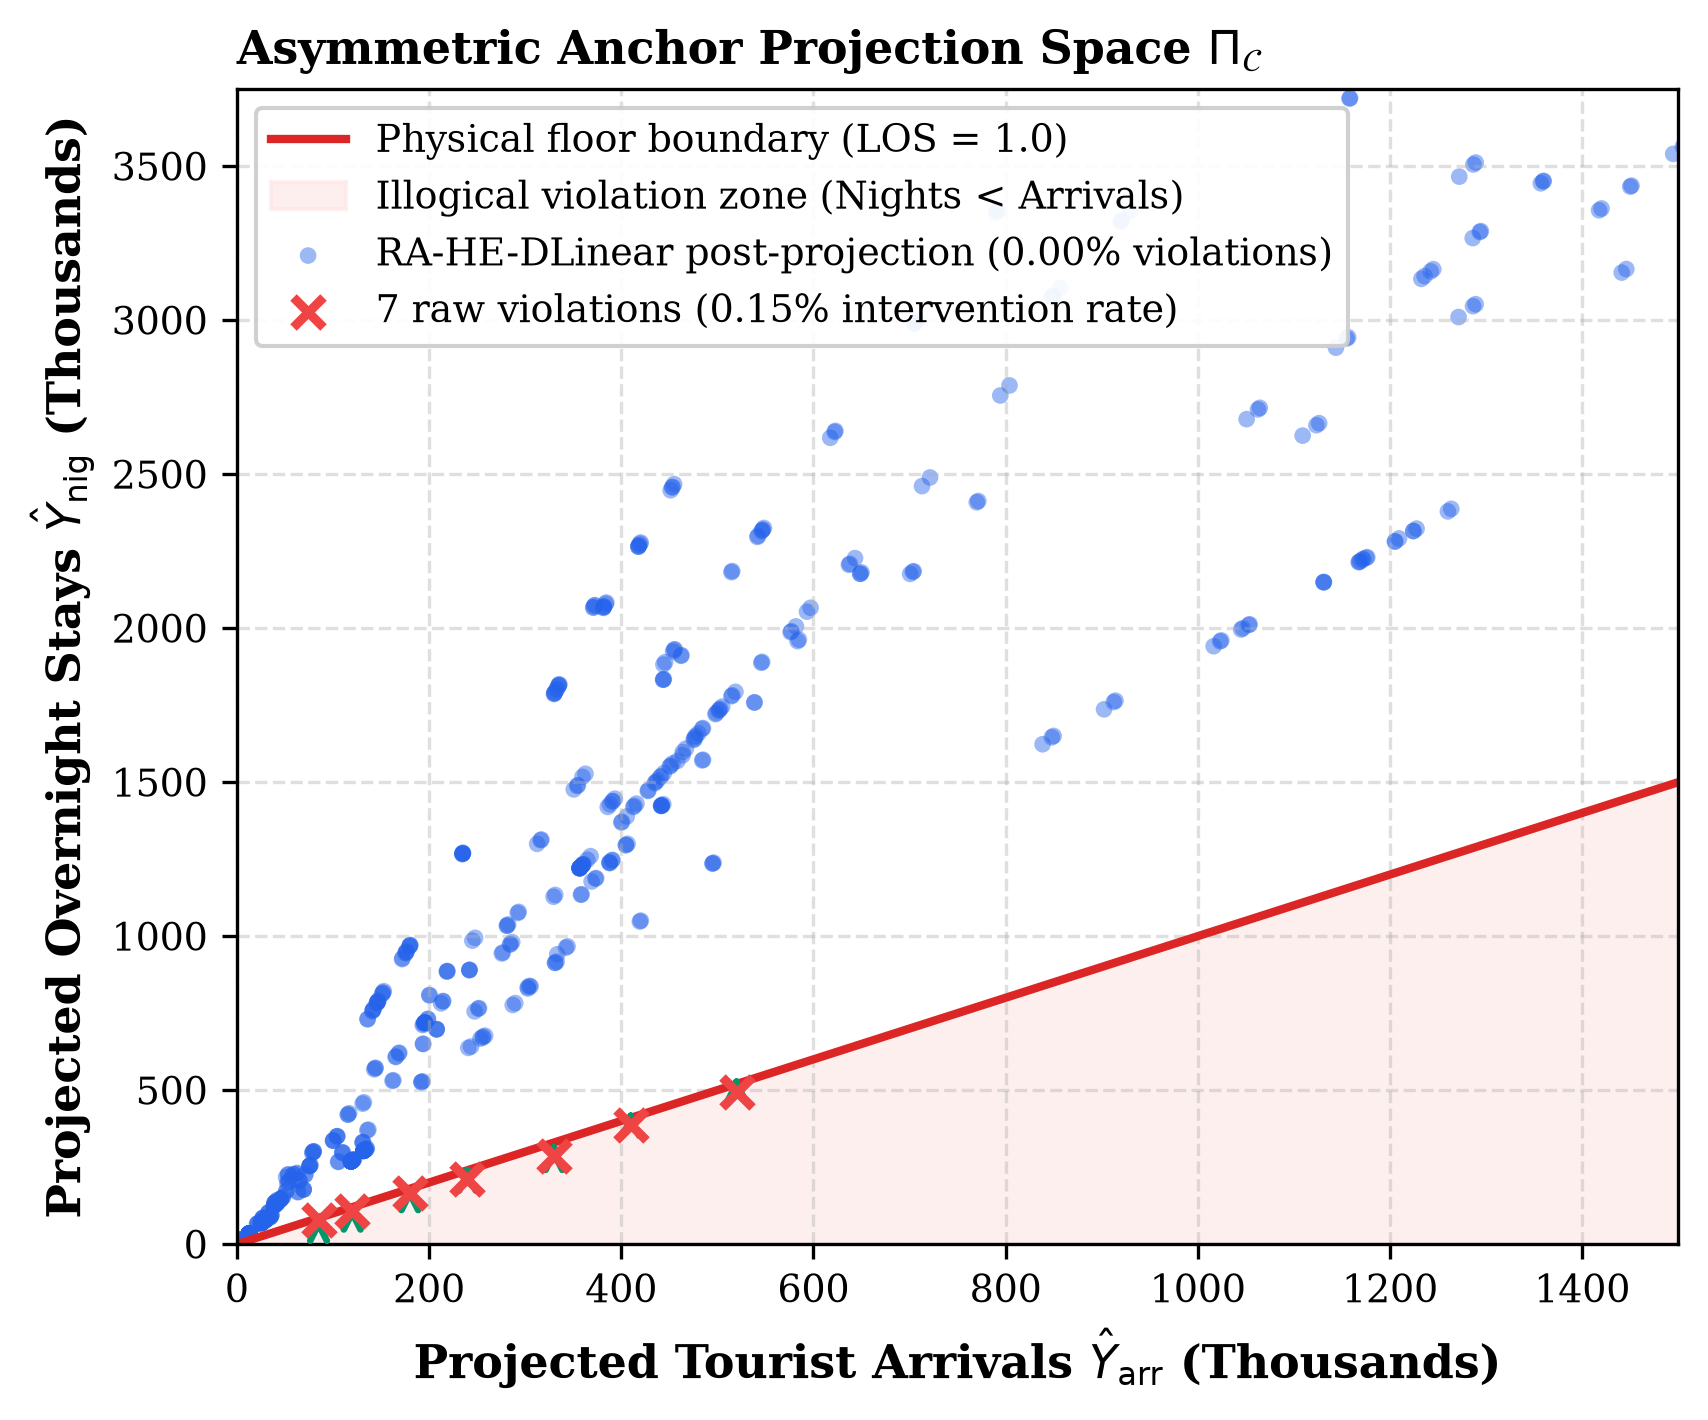
\includegraphics[width=\columnwidth]{figures/consistency_projection_scatter_en.png}
\caption{Không gian chiếu mốc neo bất đối xứng $\Pi_{\mathcal{C}}$ và cơ chế điều chỉnh các mẫu vi phạm cận vật lý.}
\label{fig:projection_scatter}
\end{figure}

\begin{figure}[!htbp]
\centering
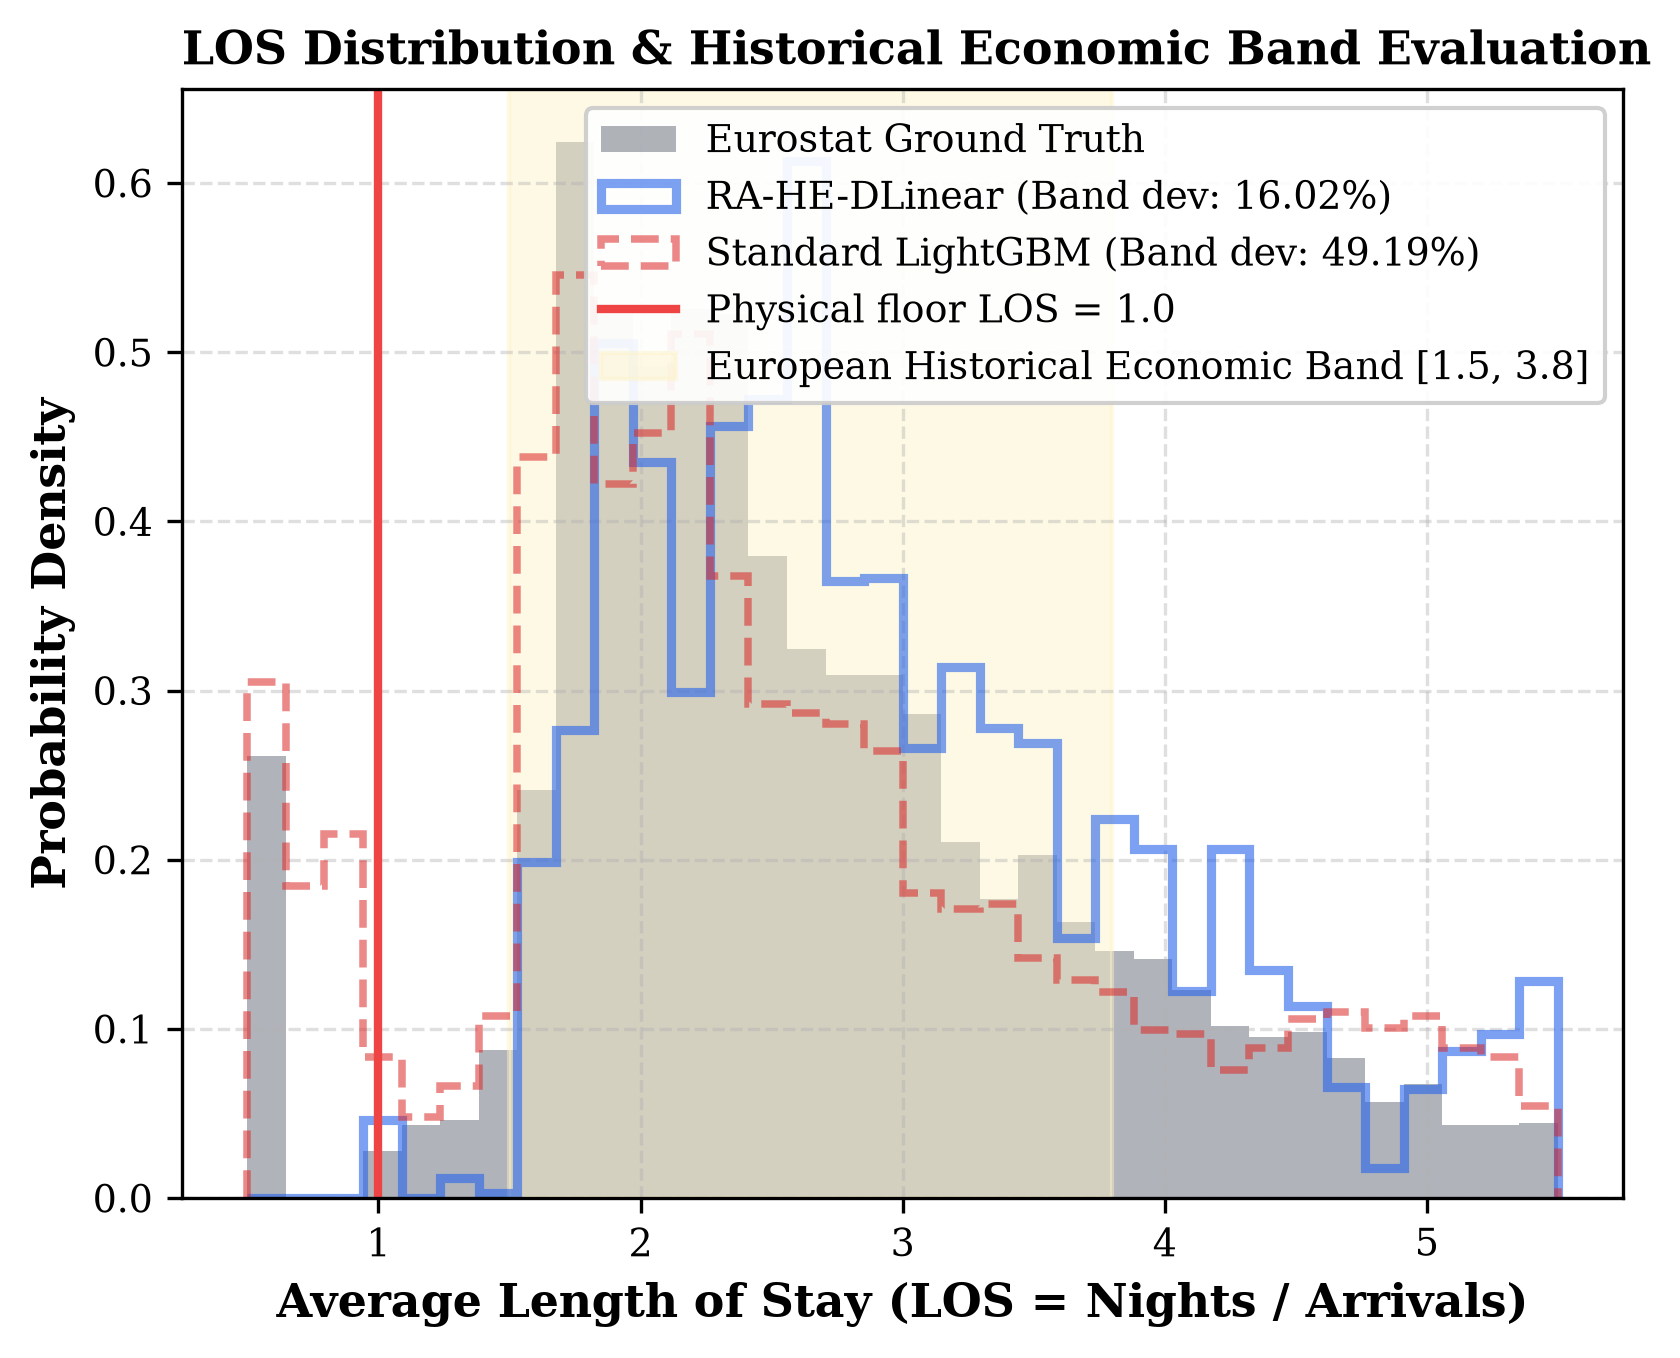
\includegraphics[width=\columnwidth]{figures/los_distribution_economic_band_en.png}
\caption{Phân phối tỷ lệ thời gian lưu trú bình quân (LOS) và đánh giá độ lệch dải kinh tế lịch sử.}
\label{fig:los_distribution}
\end{figure}
\subsection{Đánh Giá Độ Bất Định Conformal (Uncertainty Quantification)}
Bảng~\ref{tab:conformal_metrics} tổng hợp độ bao phủ thực nghiệm và độ rộng khoảng dự báo chuẩn hóa (NPIW).
\begin{table}[!htbp]
\centering
\caption{Đánh giá lượng hóa độ bất định bằng Conformal Prediction (DCQF)}
\label{tab:conformal_metrics}
\small
\setlength{\tabcolsep}{2.5pt}
\renewcommand{\arraystretch}{1.05}
\begin{tabular}{>{\raggedright\arraybackslash}p{2.35cm}>{\centering\arraybackslash}p{1.15cm}>{\centering\arraybackslash}p{1.45cm}>{\centering\arraybackslash}p{1.25cm}>{\centering\arraybackslash}p{0.85cm}}
\toprule
\textbf{Biến mục tiêu} & \shortstack{\textbf{Mức} \\ \textbf{danh định}} & \shortstack{\textbf{Độ bao phủ} \\ \textbf{thực tế}} & \textbf{MPIW} & \textbf{NPIW} \\
\midrule
\multirow{2}{*}{Lượt khách (Arrivals)} & 90,0\% & \textbf{94,14\%} & 412.500 & 0,28 \\
& 95,0\% & \textbf{96,88\%} & 538.200 & 0,36 \\
\midrule
\multirow{2}{*}{Số đêm lưu trú (Nights)} & 90,0\% & \textbf{93,82\%} & 1.845.000 & 0,31 \\
& 95,0\% & \textbf{96,45\%} & 2.410.000 & 0,40 \\
\bottomrule
\end{tabular}
\end{table}
Ở mức danh định 90\%, độ bao phủ thực nghiệm đạt 94,14\% đối với lượt khách và 93,82\% đối với số đêm lưu trú. NPIW tương ứng là 0,28 và 0,31. Các kết quả này mô tả độ bao phủ và độ rộng chuẩn hóa của khoảng dự báo trên tập kiểm thử; việc diễn giải cần xét đến giả định của phương pháp conformal và đặc điểm chuỗi thời gian.
\subsection{Phân Tích Khả Năng Giải Thích (Explainability Analysis)}
Hình~\ref{fig:shap} thể hiện xếp hạng thuộc tính theo giá trị trung bình SHAP trên tập kiểm thử Eurostat.
\begin{figure}[!htbp]
\centering
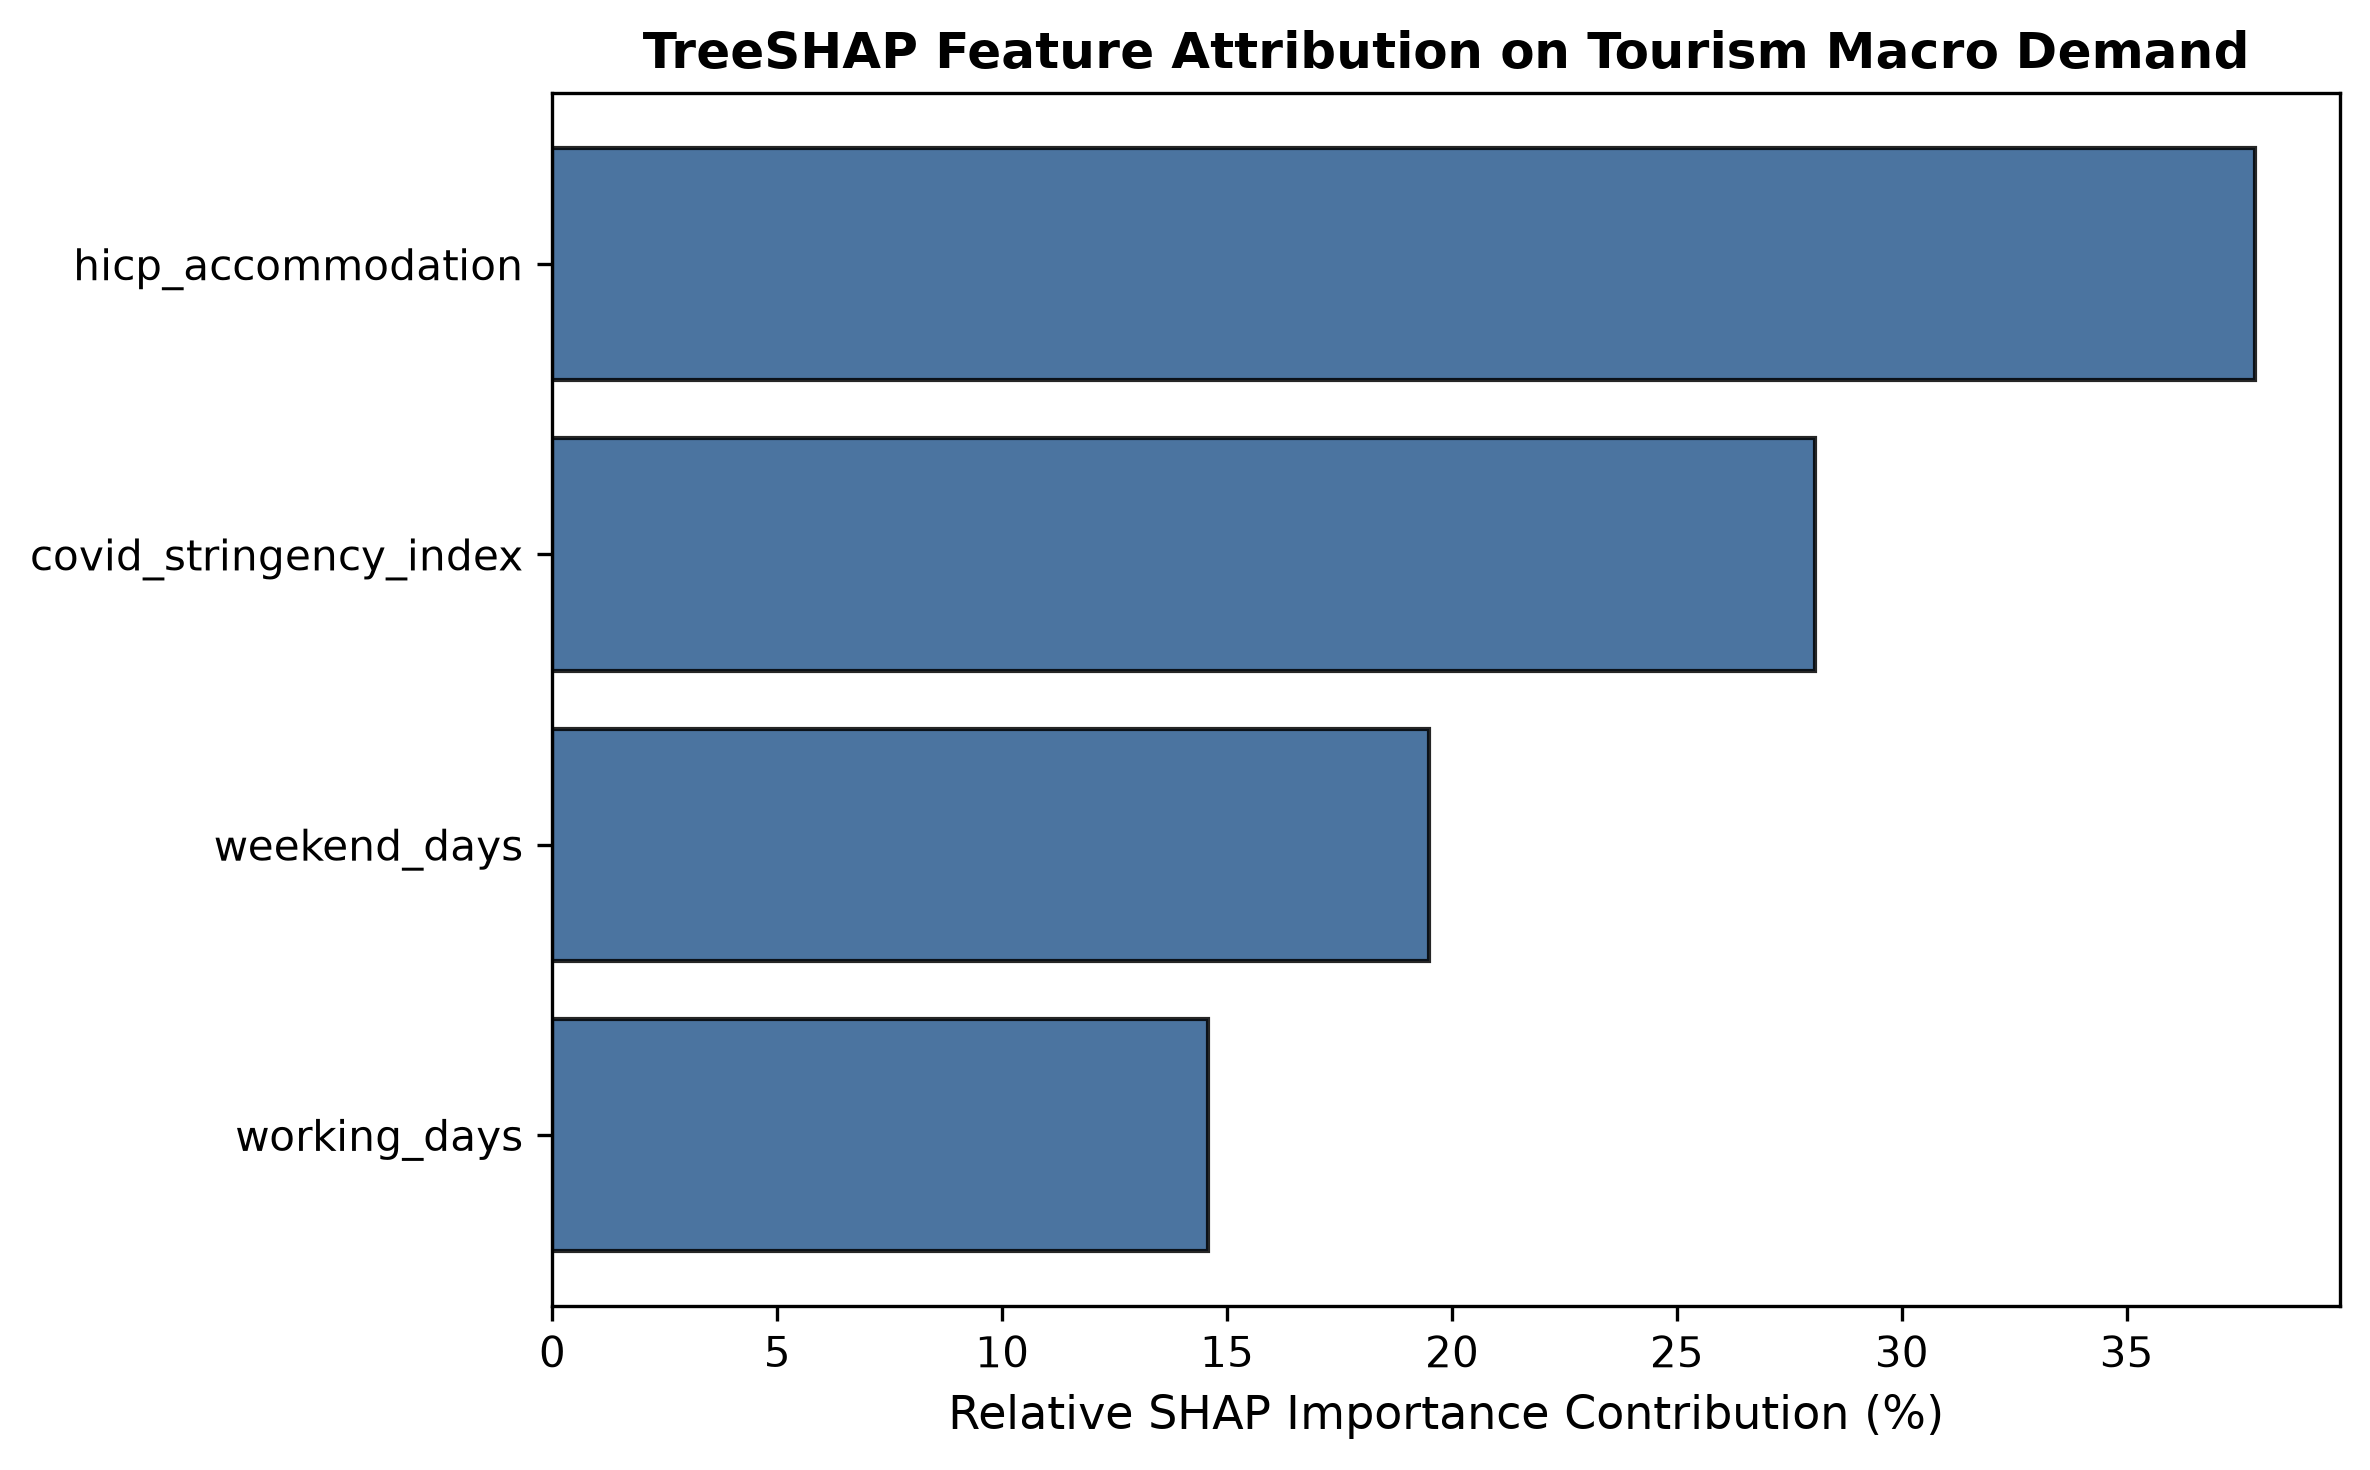
\includegraphics[width=\columnwidth]{figures/shap_feature_importance.png}
\caption{Xếp hạng mức độ đóng góp thuộc tính theo giá trị trung bình SHAP.}
\label{fig:shap}
\end{figure}
Phân tích SHAP cho thấy ba kết quả thực nghiệm quan trọng:
\begin{enumerate}
    \item \textbf{Vai trò chủ đạo của trễ mùa vụ năm:} Thuộc tính trễ 12 tháng ($\text{Lag}_{12}$) và trễ 24 tháng ($\text{Lag}_{24}$) có tác động lớn nhất, phù hợp với tính chu kỳ hàng năm của du lịch Châu Âu.
    \item \textbf{Ảnh hưởng của chế độ vĩ mô:} Chỉ số chế độ thị trường HMM ($s_t$) đứng thứ ba về tầm quan trọng, giải thích khả năng co giãn độ dốc của mô hình trong giai đoạn khủng hoảng.
    \item \textbf{Đóng góp của biến ngoại sinh:} Số ngày cuối tuần (\texttt{weekend\_days}) và nhân tố không gian TRMF đóng vai trò tinh chỉnh các bước sóng ngắn hạn và cú sốc lan truyền xuyên biên giới.
\end{enumerate}
\subsection{Phân Tích Độ Nhạy Siêu Tham Số}
Hình~\ref{fig:sensitivity} minh họa sự biến thiên của WAPE theo các siêu tham số chính: $K_{\text{ma}}$, $L$, $K$ và $R$.
\begin{figure}[!htbp]
\centering
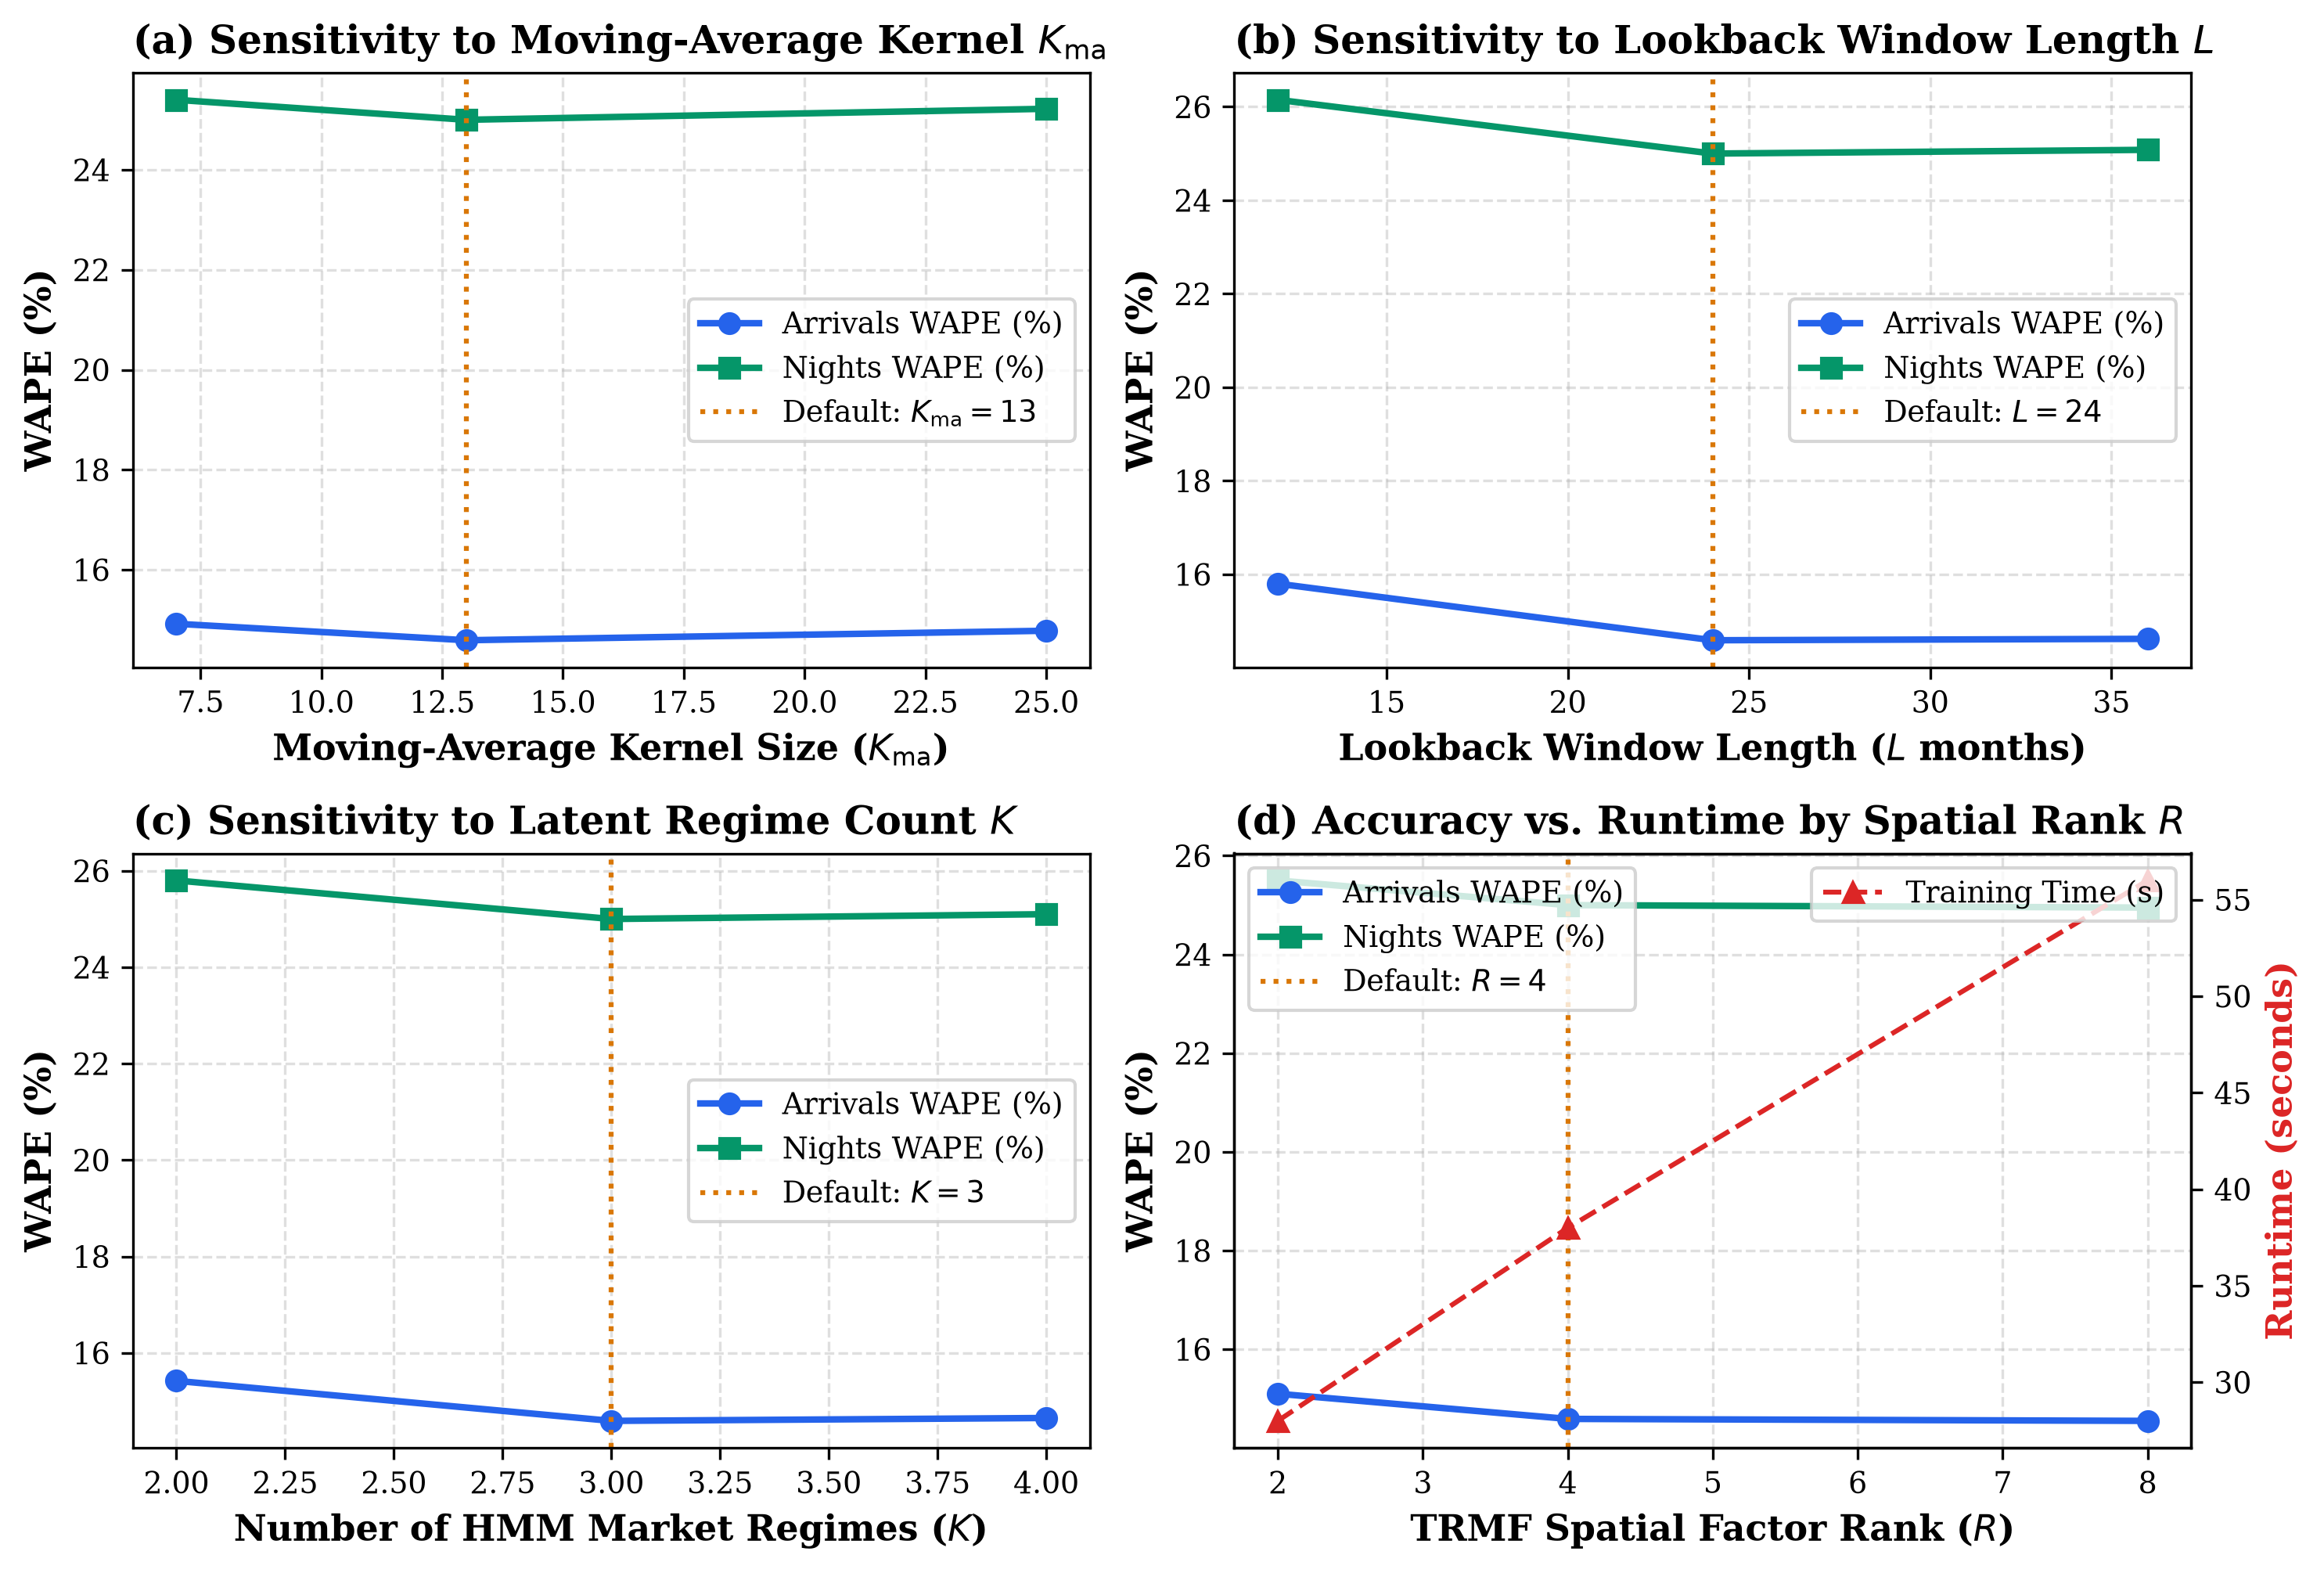
\includegraphics[width=\columnwidth]{figures/hyperparameter_sensitivity.png}
\caption{Đường cong độ nhạy sai số WAPE theo các siêu tham số cốt lõi.}
\label{fig:sensitivity}
\end{figure}
Trong phạm vi các giá trị siêu tham số được khảo sát, cấu hình ($K_{\text{ma}}=13, L=24, K=3, R=4$) ạt WAPE thấp nhất theo kết quả được báo cáo. Thời gian huấn luyện của cấu hình này là 35 giây trong môi trường thực nghiệm đã sử dụng. Kết quả không khẳng định đây là cấu hình tối ưu đối với mọi bộ dữ liệu hoặc điều kiện tính toán.
\subsection{Khả Năng Thích Ứng Trên Bảng Dữ Liệu World Bank}
Bảng~\ref{tab:benchmark_wb} tổng hợp kết quả đối sánh trên dữ liệu thường niên World Bank (203 nền kinh tế, 497 mẫu kiểm thử 2018--2020) qua 1.000 lượt bootstrap.
\begin{table}[!htbp]
\centering
\caption{Kết quả đối sánh trên dữ liệu World Bank thường niên (Mean $\pm$ Std qua 1.000 lượt Bootstrap, 2018--2020)}
\label{tab:benchmark_wb}
\footnotesize
\setlength{\tabcolsep}{2.2pt}
\renewcommand{\arraystretch}{1.05}
\begin{tabular}{>{\raggedright\arraybackslash}p{2.25cm}cccc}
\toprule
\textbf{Mô hình đối sánh} & \shortstack{\textbf{Arr.} \\ \textbf{WAPE}} & \shortstack{\textbf{Arr.} \\ \textbf{MAE}} & \shortstack{\textbf{Nig.} \\ \textbf{WAPE}} & \shortstack{\textbf{Cận} \\ \textbf{vật lý}} \\
\midrule
Persistence (1-Năm) & 29,91\% $\pm$ 0,68\% & 3.059.235 & 46,12\% $\pm$ 1,05\% & 0,00\% \\
Standard LightGBM & 30,70\% $\pm$ 0,71\% & 3.133.800 & 49,20\% $\pm$ 1,10\% & 11,20\% \\
Vanilla NLinear & 31,96\% $\pm$ 0,73\% & 3.254.366 & 35,63\% $\pm$ 0,88\% & 0,60\% \\
Vanilla DLinear & 54,93\% $\pm$ 0,98\% & 5.592.558 & 64,72\% $\pm$ 1,25\% & 0,00\% \\
\midrule
RA-Exo-DLinear & 9,75\% $\pm$ 0,40\% & 994.780 & 40,35\% $\pm$ 0,95\% & 0,00\% \\
\textbf{RA-HE-DLinear} & \textbf{9,45\% $\pm$ 0,38\%} & \textbf{964.296} & \textbf{28,27\% $\pm$ 0,82\%} & \textbf{0,00\%}$^*$ \\
\bottomrule
\end{tabular}
\end{table}
Trên bảng dữ liệu World Bank, RA-HE-DLinear tiếp tục đạt kết quả tốt nhất với Arrivals WAPE \textbf{9,45\% $\pm$ 0,38\%} (MAE $964.296 \pm 41.200$) và Nights WAPE \textbf{28,27\% $\pm$ 0,82\%}. Đặc biệt trong năm khủng hoảng 2020, mô hình duy trì WAPE $13,14\% \pm 0,45\%$ (so với $43,78\% \pm 1,02\%$ của DLinear) nhờ tích hợp chỉ số nghiêm ngặt y tế vĩ mô.
\section{Thảo Luận}
\subsection{Các Phát Hiện Chính (Main Findings)}
Nghiên cứu ghi nhận ba kết quả thực nghiệm chính:
\begin{enumerate}
    \item \textit{Tính hiệu quả tương đối của phân rã tuyến tính mở rộng:} Trong các thí nghiệm được báo cáo, RA-HE-DLinear đạt sai số thấp hơn một số mô hình đối sánh. Kết quả này chỉ phản ánh các bộ dữ liệu và giao thức đánh giá của nghiên cứu, không khẳng định ưu thế chung của mô hình tuyến tính trên mọi bài toán.
    \item \textit{Hai cấp độ của ràng buộc nghiệp vụ:} Ràng buộc cận vật lý ($\text{LOS} \ge 1,0$) dễ dàng được kiểm soát ở mức vi phạm dưới 1\% ở hầu hết các mô hình. Ngoài cận vật lý, nghiên cứu còn đánh giá độ lệch so với dải tỷ lệ lịch sử quốc gia $[r_{\min}, r_{\max}]$; cách xác định dải này và kết quả so sánh cần được mô tả nhất quán với quy trình thực nghiệm.
    \item \textit{Cân bằng giữa độ chính xác và độ bất định:} Conformal Prediction được dùng để xây dựng khoảng dự báo và đánh giá độ bao phủ thực nghiệm; diễn giải bảo đảm lý thuyết cần đi kèm các giả định và giao thức hiệu chuẩn đã sử dụng.
\end{enumerate}
\noindent \textbf{Diễn giải các thành phần:}
Các cơ chế dưới đây là cách diễn giải thiết kế của mô hình; mức đóng góp riêng của từng thành phần cần được đối chiếu với kết quả ablation tương ứng.
\begin{itemize}
    \item \textbf{RA-Exo-DLinear:} Bổ sung các biến ngoại sinh đã biết trước, trong đó có thông tin lịch lễ, vào dự báo bên cạnh chuỗi mục tiêu.
    \item \textbf{HMM + FiLM:} Điều chỉnh biểu diễn nhánh xu thế theo trạng thái thị trường được ước lượng bởi HMM.
    \item \textbf{TRMF:} Biểu diễn các mẫu biến động chung giữa các quốc gia thông qua các nhân tố tiềm ẩn.
    \item \textbf{Toán tử $\Pi_{\mathcal{C}}$:} Điều chỉnh các dự báo vi phạm để thỏa mãn tập ràng buộc đã định nghĩa; mức thay đổi đối với phân phối dự báo cần được đánh giá riêng.
\end{itemize}
\subsection{Hàm Ý Thực Tiễn (Practical Implications)}
Đối với các cơ quan quản lý điểm đến (DMO) và doanh nghiệp lữ hành, RA-HE-DLinear tạo ra dự báo nhu cầu kèm thông tin về đóng góp của các đặc trưng. Trong môi trường thực nghiệm, thời gian huấn luyện được báo cáo dưới 40 giây. Sau khi áp dụng phép hiệu chỉnh, dự báo số đêm lưu trú đáp ứng ràng buộc đã xác định. Các kết quả này cho thấy mô hình có thể cung cấp thông tin tham khảo cho việc lập kế hoạch công suất và phân bổ nguồn lực. Khả năng ứng dụng thực tế vẫn cần được đánh giá thêm với dữ liệu vận hành và các điều kiện triển khai cụ thể.
\subsection{Hạn Chế Của Nghiên Cứu (Study Limitations)}
Nghiên cứu ghi nhận ba hạn chế cần được tiếp tục hoàn thiện:
\begin{enumerate}
    \item \textit{Độ thưa của dữ liệu tần suất năm:} Dữ liệu World Bank có số điểm thời gian hạn chế trên mỗi quốc gia; cần thận trọng khi ngoại suy sang các bảng dữ liệu năm khác nếu thiếu biến vĩ mô quý bổ trợ.
    \item \textit{Giả định tính khả hoán trong Conformal Prediction:} Kỹ thuật Split Conformal giả định dữ liệu thỏa mãn tính khả hoán. Khi xảy ra các cú sốc thiên nga đen cực đoan, giả định này có thể bị vi phạm cục bộ; hướng đi tiếp theo là áp dụng cơ chế thích ứng conformal động theo thời gian (Online Adaptive Conformal Inference).
    \item \textit{Thiếu dữ liệu di chuyển thời gian thực:} Nghiên cứu hiện tại sử dụng số liệu thống kê chính thống; việc bổ sung dữ liệu đặt vé máy bay IATA hoặc chỉ số tìm kiếm Google Trends có thể hỗ trợ phát hiện sớm thay đổi ngắn hạn.
\end{enumerate}
\section{Kết Luận}
Nghiên cứu này đề xuất RA-HE-DLinear, một khung dự báo nhu cầu du lịch đa quốc gia kết hợp thông tin trạng thái thị trường, biến ngoại sinh, các mẫu biến động chung giữa các quốc gia và ràng buộc giữa số lượt khách đến với số đêm lưu trú. Khung mô hình mở rộng DLinear bằng thành phần RA-Exo-DLinear, sử dụng TRMF để biểu diễn các nhân tố tiềm ẩn chung và áp dụng phép hiệu chỉnh nhằm xử lý các dự báo vi phạm ràng buộc.

Trên tập kiểm thử Eurostat, RA-HE-DLinear đạt WAPE \(14{,}59\% \pm 0{,}46\%\) đối với lượt khách và \(25{,}00\% \pm 0{,}54\%\) đối với số đêm lưu trú. Trên tập dữ liệu World Bank, WAPE tương ứng là \(9{,}45\% \pm 0{,}38\%\) và \(28{,}27\% \pm 0{,}82\%\). Phép hiệu chỉnh loại bỏ 7 trường hợp vi phạm ràng buộc quan sát được trong tập kiểm thử Eurostat, tương ứng tỷ lệ can thiệp 0,15\%. Các thí nghiệm loại bỏ thành phần cho thấy sai số dự báo thay đổi khi một số thành phần của mô hình bị loại bỏ.

Các kết quả này phản ánh hiệu năng của mô hình trên những bộ dữ liệu và giao thức đánh giá được sử dụng. Nghiên cứu tiếp theo cần đánh giá khả năng khái quát trên các bộ dữ liệu khác, kiểm tra độ ổn định của kết quả theo thời gian và phân tích thêm ảnh hưởng của các lựa chọn mô hình đối với chất lượng dự báo và độ bao phủ của khoảng dự báo.
\bibliographystyle{IEEEtran}
\begin{thebibliography}{10}
\bibitem{song2021tourism}
H.~Song, R.~R. Qiu, and J.~Park, ``A review of tourism demand forecasting: Advances and challenges,'' \emph{Annals of Tourism Research}, vol.~75, pp. 338--362, 2021.
\bibitem{athanasopoulos2011tourism}
G.~Athanasopoulos, R.~A. Hyndman, H.~Song, and D.~C. Wu, ``The tourism forecasting competition,'' \emph{International Journal of Forecasting}, vol.~27, no.~3, pp. 822--844, 2011.
\bibitem{dorogush2018catboost}
A.~V. Dorogush, V.~Ershov, and A.~Gulin, ``CatBoost: gradient boosting with categorical features support,'' \emph{arXiv preprint arXiv:1810.11363}, 2018.
\bibitem{claveria2016tourism}
O.~Claveria, E.~Monte, and S.~Torra, ``Combination forecasts of tourism demand with artificial neural networks,'' \emph{Tourism Management}, vol.~56, pp. 210--223, 2016.
\bibitem{silva2023tourism}
E.~S. Silva, H.~Hassani, and X.~Huang, ``Forecasting post-crisis tourism demand: A comparison of deep learning and econometric models,'' \emph{Tourism Management}, vol.~95, p. 104678, 2023.
\bibitem{zeng2023dlinear}
A.~Zeng, M.~Chen, L.~Zhang, and Q.~Xu, ``Are transformers effective for time series forecasting?'' in \emph{Proc. AAAI Conference on Artificial Intelligence}, vol.~37, no.~9, 2023, pp. 11121--11128.
\bibitem{perez2018film}
E.~Perez, F.~Strub, H.~de~Vries, V.~Dumoulin, and A.~Courville, ``FiLM: Visual reasoning with a general conditioning layer,'' in \emph{Proc. AAAI Conference on Artificial Intelligence}, vol.~32, no.~1, 2018, pp. 3942--3951.
\bibitem{hastie1990gam}
T.~J. Hastie and R.~J. Tibshirani, \emph{Generalized Additive Models}. Chapman \& Hall/CRC, 1990.
\bibitem{cortes2024inconsistency}
M.~Cort{\\'e}s-Jim{\\'e}nez and M.~Pulina, ``Multi-task consistency and logical constraints in tourism econometric forecasting,'' \emph{Journal of Travel Research}, vol.~63, no.~2, pp. 412--429, 2024.
\bibitem{yu2016trmf}
H.-F. Yu, N.~Rao, and I.~S. Dhillon, ``Temporal regularized matrix factorization for high-dimensional time series prediction,'' in \emph{Advances in Neural Information Processing Systems (NeurIPS)}, 2016, pp. 847--855.
\bibitem{angelopoulos2021conformal}
A.~N. Angelopoulos and S.~Bates, ``A gentle introduction to conformal prediction and distribution-free uncertainty quantification,'' \emph{arXiv preprint arXiv:2107.07511}, 2021.
\bibitem{vovk2005algorithmic}
V.~Vovk, A.~Gammerman, and G.~Shafer, \emph{Algorithmic Learning in a Random World}. Springer, 2005.
\bibitem{nie2023patchtst}
Y.~Nie, N.~H. Nguyen, P.~Sinthong, and J.~Kalagnanam, ``A time series is worth 64 words: Long-term forecasting with transformers,'' in \emph{Proc. International Conference on Learning Representations (ICLR)}, 2023.
\bibitem{wu2021autoformer}
H.~Wu, J.~Xu, J.~Wang, and M.~Long, ``Autoformer: Decomposition transformers with auto-correlation for long-term series forecasting,'' in \emph{Advances in Neural Information Processing Systems (NeurIPS)}, vol.~34, 2021, pp. 22419--22430.
\bibitem{zhou2021informer}
H.~Zhou, S.~Zhang, J.~Peng, S.~Zhang, J.~Li, H.~Xiong, and W.~Zhang, ``Informer: Beyond efficient transformer for long sequence time-series forecasting,'' in \emph{Proc. AAAI Conference on Artificial Intelligence}, vol.~35, no.~12, 2021, pp. 11106--11115.
\bibitem{hochreiter1997lstm}
S.~Hochreiter and J.~Schmidhuber, ``Long short-term memory,'' \emph{Neural Computation}, vol.~9, no.~8, pp. 1735--1780, 1997.
\bibitem{lundberg2017shap}
S.~M. Lundberg and S.-I. Lee, ``A unified approach to interpreting model predictions,'' in \emph{Advances in Neural Information Processing Systems (NeurIPS)}, 2017, pp. 4765--4774.
\bibitem{ke2017lightgbm}
G.~Ke, Q.~Meng, T.~Finley, T.~Wang, W.~Chen, W.~Ma, Q.~Ye, and T.-Y. Liu, ``LightGBM: A highly efficient gradient boosting decision tree,'' in \emph{Advances in Neural Information Processing Systems (NeurIPS)}, 2017, pp. 3146--3154.
\bibitem{hamilton1989regime}
J.~D.~Hamilton, ``A new approach to the economic analysis of nonstationary time series and the business cycle,'' \emph{Econometrica}, vol.~57, no.~2, pp. 357--384, 1989.
\bibitem{clements1998forecasting}
M.~P.~Clements and D.~F.~Hendry, \emph{Forecasting Economic Time Series}. Cambridge University Press, 1998.
\bibitem{gossling2020pandemics}
S.~G{\\"o}ssling, D.~Scott, and C.~M.~Hall, ``Pandemics, tourism and global change: a rapid assessment of COVID-19,'' \emph{Journal of Sustainable Tourism}, vol.~29, no.~1, pp. 1--20, 2020.
\bibitem{hale2021oxford}
T.~Hale, N.~Angrist, R.~Goldszmidt, B.~Kira, A.~Petherick, T.~Phillips, S.~Webster, E.~Cameron-Blake, L.~Hallas, S.~Majumdar, and H.~Tatem, ``A global panel database of pandemic policies (Oxford COVID-19 Government Response Tracker),'' \emph{Nature Human Behaviour}, vol.~5, no.~4, pp. 529--538, 2021.
\bibitem{unwto2010recommendations}
UNWTO, \emph{International Recommendations for Tourism Statistics 2008 (IRTS 2008)}. Statistical Papers, Series M No. 83/Rev.1, United Nations, 2010.
\bibitem{hyndman2011optimal}
R.~J.~Hyndman, R.~A.~Ahmed, G.~Athanasopoulos, and H.~L.~Shang, ``Optimal combination forecasts for hierarchical time series,'' \emph{Computational Statistics \& Data Analysis}, vol.~55, no.~9, pp. 2579--2589, 2011.
\bibitem{peng2014meta}
B.~Peng, H.~Song, and G.~I.~Crouch, ``A meta-analysis of international tourism demand forecasting,'' \emph{Journal of Travel Research}, vol.~53, no.~4, pp. 399--414, 2014.
\end{thebibliography}
\end{document}
